\chapter{The Simulation Library}
\label{cha:the-simulation-library}

{\opp} has a rich C++ class library which you can use when implementing
simple modules. A quick overview of the areas supported by the
simulation library:
\begin{itemize}
  \item{sending and receiving messages, scheduling and cancelling
    events, terminating the module or the simulation: member functions
    of \cclass{cSimpleModule}}
  \item{events, messages, network packets: the
    \cclass{cMessage} and \cclass{cPacket} classes}
  \item{random number generation: \fname{normal()},
    \fname{exponential()}, etc.}
  \item{access to module gates and parameters: member functions of
    \cclass{cModule} (base class for
    \cclass{cSimpleModule}); \cclass{cPar} and
    \cclass{cGate} classes}
  \item{accessing other modules in the network: member functions of \cclass{cModule}
    and \cclass{cGate}}
  \item{storing data in containers: \cclass{cArray},
    \cclass{cQueue}, \cclass{cBag} and
    \cclass{cLinkedList} classes}
  \item{discovering network topology and support routing: \cclass{cTopology} class}
  \item{recording statistics into file: \cclass{cOutVector} class}
  \item{collecting simple statistics: \cclass{cStdDev} and
    \cclass{cWeightedStddev} classes}
  \item{distribution estimation: \cclass{cLongHistogram},
    \cclass{cDoubleHistogram},
    \cclass{cVarHistogram}, \cclass{cPSquare},
    \cclass{cKSplit} classes}
  \item{making variables inspectable in the graphical user interface
    (Tkenv): the \fmac{WATCH()} macro (\cclass{cWatch} class)}
  \item{sending debug output to and prompting for user input in the graphical
    user interface (Tkenv\index{Tkenv}): the ev\index{ev} object (\cclass{cEnvir} class)}
\end{itemize}





\section{Class library conventions}

\textbf{Base class}


Classes in the {\opp} simulation library are derived from \cclass{cObject}.
Functionality and conventions that come from \cclass{cObject}:
\begin{itemize}
  \item{name attribute}
  \item{\fname{className()} member and other member functions giving textual
    information about the object}
  \item{conventions for assignment, copying, duplicating the object}
  \item{ownership\index{ownership} control for containers derived from \cclass{cObject}}
  \item{support for traversing the object tree}
  \item{support for inspecting the object in graphical user interfaces
    (Tkenv)}
  \item{support for automatic cleanup (garbage collection) at the end
    of the simulation}
\end{itemize}


Classes inherit and redefine several \cclass{cObject} member functions;
in the following we'll discuss some of the practically important
ones.


\textbf{Setting and getting attributes}


Member functions that set and query object attributes follow
consistent naming. The setter member function has the form setSomething(...)
and its getter counterpart is named something(), i.e. the ''get''
verb found in Java and some other libraries is omitted for brevity.
For example, the \textit{length} attribute of the \cclass{cMessage} class can
be set and read like this:

\begin{verbatim}
msg->setLength( 1024 );
length = msg->length();
\end{verbatim}


\textbf{className()}


For each class, the \fname{className()} member function returns the class
name as a string:

\begin{verbatim}
const char *classname = msg->className(); // returns "cMessage"
\end{verbatim}

\textbf{Name attribute}


An object can be assigned a name (a character string). The name
string is the first argument to the constructor of every class,
and it defaults to NULL (no name string). If you supply a name
string, the object will make its own copy (\fname{strdup()}). As an example,
you can create a message object like this:

\begin{verbatim}
cMessage *mymsg = new cMessage("mymsg");
\end{verbatim}


You can also set the name after the object has been created:

\begin{verbatim}
mymsg->setName("mymsg");
\end{verbatim}

You can get a pointer to the internally stored copy of the name
string like this:

\begin{verbatim}
const char *name = mymsg->name(); // --> returns ptr to internal copy
                                  // of "mymsg"
\end{verbatim}


For convenience and efficiency reasons, the empty string ''''
and NULL are treated as equivalent by library objects: ''''
is stored as NULL (so that it does not consume heap), but it
is returned as '''' (so that it is easier to print
out etc). Thus, if you create a message object with either NULL
or '''' as name, it will be stored as NULL and \fname{name()}
will return a pointer to '''', a static string:

\begin{verbatim}
cMessage *msg = new cMessage(NULL, <additional args>);
const char *str = msg->name(); // --> returns ptr to  ""
\end{verbatim}


\textbf{fullName() and fullPath()}


Objects have two more member functions which return other sort
of names based on the name attribute: \fname{fullName()} and \fname{fullPath()}.

Suppose we have a module in the network university\_lan, compound
module fddi\_ring, simple module station[10]. If you call the functions
on the simple module object (\cclass{cSimpleModule} inherits from
\cclass{cObject}, too), the functions will return these values:

\begin{verbatim}
ev << module->name(); // --> "station"
ev << module->fullName(); // --> "station[10]"
ev << module->fullPath(); // --> "university_lan.fddi_ring.station[10]"
\end{verbatim}



These functions work for any object. For example, a local object
inside the module would produce results like this:


\begin{verbatim}
void FDDIStation::activity()
{
    cQueue buffer("buffer");
    ev << buffer->fullPath(); // --> "university_lan.fddi_ring.
                              // station[10].buffer"
}
\end{verbatim}



\fname{fullName()} and \fname{fullPath()}, together with
\fname{className()} can be used for example to generate informative
error messages.

Be aware that \fname{fullName()} and \fname{fullPath()} return
pointers to static buffers. Each call will overwrite the previous
content of the buffer, so for example you shouldn't put two calls in a
single \fname{printf()} statement:

\begin{verbatim}
ev.printf("object1 is '%s', object2 is '%s'\n",
          object1->fullPath(),
          object2->fullPath()
         ); // WRONG! Same string is printed twice!!!
\end{verbatim}


\textbf{Copying and duplicating objects}


The \fname{dup()} member function creates an exact copy of the
object\index{object!copy}, duplicating\index{object!duplication}
contained objects also if necessary. This is especially useful in the
case of message objects. \fname{dup()} returns a pointer of type
\cclass[cObject]{cObject*}, so it needs to be cast to the proper type:

\begin{verbatim}
cMessage *copyMsg = (cMessage *) msg->dup();
\end{verbatim}


\fname{dup()} works through calling the copy constructor, which in
turn relies on the assignment operator between objects.
\fname{operator=()} can be used to copy contents of an object into
another object of the same type. The copying is done properly; object
contained in the object will also be duplicated if necessary. For
various reasons, \fname{operator=()} does not copy the name string;
the copy constructor\index{copy constructor} does it.


\textbf{Iterators}


There are several container classes in the library (\cclass{cQueue},
\cclass{cArray} etc.) For many of them, there is a corresponding
iterator class that you can use to loop through the objects stored in
the container.

For example:

\begin{verbatim}
cQueue queue;

//..
for (cQueueIterator queueIter(queue); !queueIter.end(); queueIter++)
{
    cObject *containedObject = queueIter();
}
\end{verbatim}


\textbf{Ownership control}


By default, if a container object is destroyed, it destroys the
contained objects too. If you call \fname{dup()}, the contained
objects are duplicated too for the new container. This is done so
because contained objects are owned by the container; ownership is
defined as the right/duty of deallocation. However, there is a
fine-grain ownership control\index{ownership} mechanism built
in which allows you to specify on per-object basis whether you want
objects to be owned by the container or not; by calling the
\fname{takeOwnership()} member function with false, you tell the
container that you don't want it to become the owner of objects that
will be inserted in the future.

The ownership mechanism is discussed in detail in
\ref{sec:ch-sim-lib:ownership-management}


\section{Utilities}

\textbf{Tracing}


The tracing feature will be used extensively in the code examples,
so it is shortly introduced here. It will be covered in detail
in a later section.

The ev\index{ev} object represents the user interface of the
simulation.  You can send debugging output to ev with the C++-style
output operators:

\begin{verbatim}
ev << "packet received, sequence number is "
   << seq_num << endl;
\end{verbatim}

An alternative solution is \fname{ev.printf()}:

\begin{verbatim}
ev.printf("packet received, sequence number is %d\n", seq_num);
\end{verbatim}

\textbf{Simulation time conversion}


There are utility functions which convert simulation
time\index{simulation time} (\cclass{simtime\_t}) to a printable string
(like ''3s 130ms 230us'') and vica versa.


The \fname{simtimeToStr()} function converts a \cclass{simtime\_t}
(passed in the first arg) to textual form. The result is placed into
the buffer pointed to by the second arg. If the second arg is omitted
or it is NULL, \fname{simtimeToStr()} will place the result into a
static buffer which is overwritten with each call:

\begin{verbatim}
char buf[32];
ev.printf("t1=%s, t2=%s\n", simtimeToStr(t1), simTimeToStr(t2,buf));
\end{verbatim}


The \fname{strToSimtime()} function parses a time specification passed
in a string, and returns a \cclass{simtime\_t}. If the string cannot
be entirely interpreted, -1 is returned:

\begin{verbatim}
simtime_t t = strToSimtime("30s 152ms");
\end{verbatim}

Another variant, \fname{strToSimtime0()} can be used if the time
string is a substring in a larger string. Instead of taking a char*,
it takes a reference to char* (char*\&) as the first argument.  The
function sets the pointer to the first character that could not be
interpreted as part of the time string, and returns the value. It
never returns -1; if nothing at the beginning of the string looked
like simulation time, it returns 0.

\begin{verbatim}
const char *s = ''30s 152ms and some rubbish'';

simtime_t t = strToSimtime0(s); // now s points to "and some rubbish"
\end{verbatim}

\textbf{Utility \texttt{<}string.h\texttt{>} functions}

\begin{sloppypar}
The \fname{opp\_strdup()}, \fname{opp\_strcpy()}, \fname{opp\_strcmp()}
functions are the same as their \texttt{<string.h>} equivalents,
except that they treat NULL and the empty string ('''') as identical,
and \fname{opp\_str\-dup()} uses operator new instead of
\fname{malloc()}.
\end{sloppypar}

The \fname{opp\_concat()} function might also be useful, for example
in constructing object names. It takes up to four const char *
pointers, concatenates them in a static buffer and returns a pointer
to the result. The result's length shouldn't exceed 255 characters.





\section{Messages and packets}

\subsection{The cMessage class}

\cclass{cMessage} is a central class in {\opp}. Objects of \cclass{cMessage} and
subclasses may model a number of things: events\index{events};
messages\index{message}; packets\index{packets},
frames\index{frames}, cells\index{cells}, bits or signals travelling
in a network; entities travelling in a system and so on.


\textbf{Attributes}


A \cclass{cMessage} object has number of attributes. Some are used by
the simulation kernel, others are provided just for the convenience
of the simulation programmer. A more-or-less complete list:
\begin{itemize}
  \item{The \textit{name} attribute is inherited from \cclass{cObject}.}
  \item{The \textit{message kind} attribute is supposed to carry some message
    type information. Zero and positive values can be freely used
    for any purpose. Negative values are reserved for use by the
    {\opp} simulation library; especially, MK\_PACKET (-1) and MK\_INFO
    (-2) are used to denote that the message is a network packet
    (see the \cclass{cPacket} class later).}
  \item{The \textit{length} attribute (understood in bits) is used to compute
    transmission delay when the message travels through a connection
    that has an assigned data rate.}
  \item{The \textit{bit error flag} attribute is set to true by the simulation
    kernel with a probability of $1-(1-\textit{ber})^{\mathit{length}}$ when the
    message is sent through a connection that has an assigned bit
    error rate (\textit{ber}).}
  \item{The \textit{priority} attribute is used by the simulation kernel to
    order messages in the message queue (FES) that have the same
    arrival time values.}
  \item{The \textit{time stamp} attribute is not used by the simulation kernel;
    you can use it for purposes like remembering the time when the
    message was enqueued or re-sent.}
  \item{Other attributes and data members make simulation programming
    easier, they will be discussed later: \textit{parameter list}, \textit{encapsulated
      message}, \textit{context pointer}.}
  \item{A number of read-only attributes store information about the
    message's (last) sending/scheduling: \textit{source/destination module
      and gate}, \textit{sending (scheduling) and arrival time}. They are
    mostly used by the simulation kernel while the message is in
    the FES, but the information is still in the message object when
    a module receives the message.}
\end{itemize}


\textbf{Basic usage}


A \cclass{cMessage} object can be created in the following way:

\begin{verbatim}
cMessage *msg = new cMessage("msg-name", kind, length,
                             priority, errorflag);
\end{verbatim}

\index{message!data members}

The kind, length, and priority are integers, and errorflag is boolean.
All arguments have default values, so the following initializations
are also valid:

\begin{verbatim}
cMessage *msg1 = new cMessage;
cMessage *msg2 = new cMessage("data-packet", DATAPACKET_KIND, 8*1500 );
\end{verbatim}


Once a message has been created, its data members can be changed by the following functions:

\begin{verbatim}
msg->setKind( kind );
msg->setLength( length );
msg->setPriority( priority );
msg->setBitError( err );
msg->setTimestamp();
msg->setTimestamp( simtime );
\end{verbatim}


With these functions the user can set the message
kind\index{message!kind}, the message length\index{message@length},
the priority\index{message!priority}, the error
flag\index{message!error flag} and the time stamp\index{message!time
  stamp}. The \fname{setTimeStamp()} function without any argument
sets the time stamp to the current simulation time.


The values can be obtained by the following functions:

\begin{verbatim}
int k       = msg->kind();
int p       = msg->priority();
int l       = msg->length();
bool b      = msg->hasBitError();
simtime_t t = msg->timestamp();
\end{verbatim}


\textbf{Duplicating messages}

\index{message!duplication}

It is often needed to duplicate a message (for example, send
one and keep a copy). This can be done in the standard ways as
for any other {\opp} object:

\begin{verbatim}
cMessage *copy1 = (cMessage *) msg->dup();
cMessage *copy2 = new cMessage( *msg );
\end{verbatim}


The two are equivalent. The resulting message is an exact copy
of the original, including message parameters (\cclass{cPar} or other
object types) and encapsulated messages.




\subsection{Message encapsulation}

It is often necessary to encapsulate a
message\index{message!encapsulation} into another when you're modeling
layered protocols of computer networks. Although you can encapsulate
messages by adding them to the parameter list, there's a better way.


The \fname{encapsulate()} function encapsulates a message
into another one. The length of the message will grow by the length of
the encapsulated message. An exception: when the encapsulating (outer)
message has zero length, {\opp} assumes it is not a real packet but
some out-of-band signal, so its length is left at zero.

\begin{verbatim}
cMessage *userdata = new cMessage("userdata");

userdata->setLength(8*2000);
cMessage *tcpseg = new cMessage("tcp");
tcpseg->setLength(8*24);
tcpseg->encapsulate(userdata);
ev << tcpseg->length() << endl; // --> 8*2024 = 16192
\end{verbatim}


A message can only hold one encapsulated message at a time. The
second \fname{encapsulate()} call will result in an error. It is also
an error if the message to be encapsulated isn't owned by the
module.

You can get back the encapsulated message by \fname{decapsulate()}:

\begin{verbatim}
cMessage *userdata = tcpseg->decapsulate();
\end{verbatim}

\fname{decapsulate()} will decrease the length of the message accordingly,
except if it was zero. If the length would become negative, an
error occurs.


The \fname{encapsulatedMsg()} function returns a pointer to the encapsulated
message, or NULL if no message was encapsulated.





\subsection{Information about the last sending}

There are several variables in \cclass{cMessage} that store
information about the last time the message was sent or
scheduled. These variables can only be read.

\fname{isSelfMessage()} returns true if the message has been scheduled
(\fname{scheduleAt()}) as opposed to being sent with one of the
\fname{send...()} methods.

\begin{Verbatim}[commandchars=\\\{\}]
bool \fname{isSelfMessage()}
\end{Verbatim}

The following methods can tell where the message came from and
where it arrived (will arrive).

\begin{Verbatim}[commandchars=\\\{\}]
int \fname{senderModuleId()};
int \fname{senderGateId()};
int \fname{arrivalModuleId()};
int \fname{arrivalGateId()};
\end{Verbatim}

The following two methods are just convenience functions that
combine module id and gate id into a gate object pointer.

\begin{Verbatim}[commandchars=\\\{\}]
cGate *\fname{senderGate()};
cGate *\fname{arrivalGate()};
\end{Verbatim}

And there are further convenience functions to tell whether
the message arrived on a specific gate given with id or
name+index.

\begin{Verbatim}[commandchars=\\\{\}]
bool \fname[arrivedOn()]{arrivedOn}(int id);
bool \fname{arrivedOn}(const char *gname, int gindex=0);
\end{Verbatim}

The following methods return message creation time and the last sending
and arrival times.

\begin{Verbatim}[commandchars=\\\{\}]
simtime_t \fname{creationTime()}
simtime_t \fname{sendingTime()};
simtime_t \fname{arrivalTime()};
\end{Verbatim}




\subsection{Context pointer}

\cclass{cMessage} contains a void* pointer which is
set/returned by the \fname{setContextPointer()} and
\fname{contextPointer()} functions:

\begin{verbatim}
void *context =...;
msg->setContextPointer( context );
void *context2 = msg->contextPointer();
\end{verbatim}


It can be used for any purpose by the simulation programmer.
It is not used by the simulation kernel, and it is treated as
a mere pointer (no memory management is done on it).

Intended purpose: a module which schedules several self-messages
(timers) will need to identify a self-message when it arrives back to
the module, ie. the module will have to determine which timer went off
and what to do then. The context pointer\index{context pointer} can be
made to point at a data structure kept by the module which can carry
enough ''context'' information about the event.





\subsection{The cPacket class}


The \cclass{cPacket} class is derived from \cclass{cMessage}. It is intended as
a base for all messages that model packets or frames in a telecommunications
network.

\cclass{cPacket} adds two new data members to \cclass{cMessage}:
\textit{protocol} and \textit{PDU} type (packet, frame or event type).
Both are short integers, and are handled by the following member
functions:

\begin{Verbatim}[commandchars=\\\{\}]
short \fname{protocol()};
short \fname{pdu()};
setProtocol(short p);
setPdu(short p);
\end{Verbatim}

Acceptable message kind values are:
\begin{itemize}
\item{MK\_PACKET}\index{MK\_PACKET}
\item{MK\_INFO}\index{MK\_INFO}
\end{itemize}

The \cclass{cPacket} constructor sets the message kind to \fname{MK\_PACKET}.
Both \fname{MK\_PACKET} and \fname{MK\_INFO} are defined as negative integers.
(Remember, negative message kind values are reserved for the simulation library.)

The protocol and PDU fields would ideally take a value from the \fname{protocol.h}
header in the simulation library. The contents of \fname{protocol.h}
is currently experimental; comments and contributions are welcome.



\subsection{Attaching parameters and objects}

If you want to add parameters or objects to a message, the preferred
way to do that is via message definitions, described in chapter
\ref{cha:message-definitions}.

\textbf{Attaching objects}

The \cclass{cMessage} class has an internal \cclass{cArray} object which can
carry objects\index{message!attaching objects}. Only objects
that are derived from \cclass{cObject} (most {\opp} classes are so) can be attached.
The \fname{addObject()}, \fname{getObject()}, \fname{hasObject()},
\fname{removeObject()} methods use the object name
as the key to the array. An example:

\begin{verbatim}
cLongHistogram *pklen_distr = new cLongHistogram("pklen_distr");
msg->addObject( pklen_distr );
...
if (msg->hasObject("pklen_distr"))
{
   cLongHistogram *pklen_distr =
       (cLongHistogram *) msg->getObject("pklen_distr");
   ...
}
\end{verbatim}

You should take care that names of the attached objects do not
clash with each other or with \cclass{cPar} parameter names
(see next section).
If you do not attach anything to the message and do not call the
\fname{parList()} function, the internal \cclass{cArray} object
will not be created.
This saves both storage and execution time.

You can attach non-object types (or non-\cclass{cObject} objects) to
the message\index{message!attaching non-object types} by using
\cclass{cPar}'s void* pointer 'P') type (see later in the description
of \cclass{cPar}). An example:

\begin{verbatim}
struct conn_t *conn = new conn_t; // conn_t is a C struct
msg->addPar("conn") = (void *) conn;
msg->par("conn").configPointer(NULL,NULL,sizeof(struct conn_t));
\end{verbatim}



\textbf{Attaching parameters}

The old way of attaching parameters is adding \cclass{cPar} objects.
There are several downsides of this approach, the most notable ones
being large memory and runtime overhead. It has been reported that
using \cclass{cPar} message parameters might account for a large
part of execution time, sometimes as much as 80\%. (This depends
on how many parameters you use.) Therefore it is recommended
that you use message definitions \ref{cha:message-definitions}
which adds the required parameters to the new message class
as \ttt{int}, \ttt{long}, \ttt{bool} etc. class members, via
subclassing.

However, if you still need to use cPars, here's a short summary
how you can do it.
You add a new parameter to the message with the
\fname{addPar()} member function, and get back a reference
to the parameter object with the \fname{par()} member function.
\fname{hasPar()} tells you if the message has a
given parameter or not.

Examples:

\begin{verbatim}
msg->addPar("dest_addr");
msg->par("dest_addr") = 168;

if (msg->hasPar("dest_addr")) {
   long dest_addr = msg->par("dest_addr");
   ...
}
\end{verbatim}

Message parameters can be accessed also by index in the parameter
array. The \fname{findPar()} function returns the index of a parameter
or -1 if the parameter cannot be found. The parameter can then be
accessed using an overloaded \fname{par()} function.

\begin{verbatim}
int index = msg->findPar("dest_addr");
long dest_addr = msg->par(index);
\end{verbatim}


\section{Sending and receiving messages}

\subsection{Sending messages}

Once the message has been created, it can be sent through an
output gate\index{output!gate} using one of these functions:

\fname[send()]{send(cMessage *msg, const char *gate\_name, int index);}\\
\fname[send()]{send(cMessage *msg, int gate)};



For the first function, the argument \fname{gate\_name} is the name of
the gate the message has to be sent through. If this gate is
a vector gate, index determines though which particular output
gate this has to be done; otherwise, the index argument is not
needed.

The second function uses the gate number and because it does
not have to search through the gate array, it is faster than
the first one.


Examples:

\begin{verbatim}
send( new cMessage("token"), "out-gate");
send( new cMessage("token"), "vectorgate", i);

int out_gate_id = findGate("out-gate");
for (i=0; i<n; i++)
{
  send( new cMessage("packet"), out_gate_id);
  wait(in_time);
}
\end{verbatim}


All message sending functions check that you actually own the message
you are about to send. If the message is with another module,
currently scheduled or in a queue etc., you'll get a runtime error.
(The feature does not increase runtime overhead significantly, because
it uses the object ownership\index{ownership} management (described in
Section \ref{sec:ch-sim-lib:ownership-management});
it merely checks that the owner of the message is the module which
wants to send it.)





\subsection{Delayed sending}

It is often needed to model a delay (processing time, etc.) immediately
followed by message sending. In {\opp}, it is possible to implement
it like this:

\begin{verbatim}
wait( some_delay );
send( msg, "outgate" );
\end{verbatim}


If the module needs to react to messages that arrive during the delay,
\fname{wait()} cannot be used and the timer mechanism described in
Section \ref{sec:ch-sim-lib:self-messages}, ``Self-messages'', would
need to be employed.


However, there is a more straightforward method than the above two,
and this is delayed sending\index{delayed sending}. Delayed sending
can be done with one of these functions:

\fname[sendDelayed()]{sendDelayed(cMessage *msg, double delay, const char *gate\_name, int index);}\\
\fname[sendDelayed()]{sendDelayed(cMessage *msg, double delay, int gate\_id);}


The arguments are the same as for \fname{send()}, except for the extra \textit{delay}
parameter. The effect of the function is the same as if the module
had kept the message for the delay interval and sent it afterwards.
That is, the sending time of the message will be the current
simulation time (time at the \fname{sendDelayed()} call) plus the delay.
The delay value must be nonnegative.

Example:

\begin{verbatim}
sendDelayed( new cMessage("token"), 0.005, "out-gate");
\end{verbatim}






\subsection{Direct message sending}

Sometimes it is necessary or convenient to ignore gates/connections
and send a message directly to a remote destination module. The \fname{sendDirect()}
function does that, and it takes the pointer of the remote module
(\cclass{cModule} *). You can also specify a delay and an input gate of
the destination module.

\begin{verbatim}
cModule *destinationmodule =...;
double delay = truncnormal(0.005, 0.0001);
sendDirect( new cMessage, delay, destinationmodule, "in" );
\end{verbatim}

The destination module receives the message as if it was sent
''normally''.



\subsection{Receiving messages}

\textbf{With activity() only!} The message receiving functions can
only be used in the \fname{activity()} function,
\fname{handleMessage()} gets the messages in its argument list.

A message can be received by a number of functions, the most
general one is the \fname{receive()} function:

\begin{verbatim}
cMessage *msg = receive();
\end{verbatim}

Simple module objects contain a built-in queue object called
putAsideQueue\index{putAsideQueue}. The put-aside queue is used by
some of the message-receiving functions.

There are two groups of functions that receive messages:
\begin{itemize}
\item{\fname{receive()}, \fname{receiveOn()}}
\item{\fname{receiveNew()}, \fname{receiveNewOn()}}
\end{itemize}

The functions \fname{receive()}/\fname{receiveOn()}check the put-aside queue
first and try to return a message from it. Only if they do not
find an appropriate message in the put-aside queue, will wait
for new messages.

The functions \fname{receiveNew()}/\fname{receiveNewOn()} wait for new messages,
ignoring the put-aside queue.

Furthermore, the ...On() functions expect messages to arrive on a
specific gate. Messages that arrive on another gate are inserted into
the put-aside queue. The On-less versions accept any message.

Since the \fname{receive()} and \fname{receiveOn()} return messages
also from the put-aside queue, the arrival times of messages they
return can be less than the current simulation time. A naive (and also
incorrect) approach to check whether a message is a new one or it has
been retrieved from the putaside-queue could be the following:

\begin{verbatim}
cMessage *msg = receive();

if (msg->arrivalTime()<simTime()) // not correct! several events may
                                  // occur at the same simulation time
{
  // handle msg as an old message
}
\end{verbatim}


The correct way to do this is to check the putaside-queue:

\begin{verbatim}
bool queue_was_empty = putAsideQueue.empty();
cMessage *msg = receive();

if (!queue_was_empty)
{
  // handle msg as an old message
}
\end{verbatim}


To discard the contents of the put-aside queue, one could use
the following code:

\begin{verbatim}
while (!putAsideQueue.empty())
  delete receive();
\end{verbatim}


To demonstrate \fname{receiveOn()}, the following code fragment waits
for a message on one specific input gate and discards all messages
that arrived on other gates in the meanwhile:

\begin{verbatim}
cMessage *msg = receiveNewOn("important_input_gate");
while (!putAsideQueue.empty())
  delete receive();
\end{verbatim}


The above code is almost equivalent to the following, except
that it preserves the previous contents of the put-aside queue:

\begin{verbatim}
cMessage *msg;
for(;;)
{
  msg = receiveNew();
  if (msg->arrivedOn("important_input_gate"))
    break;
  delete msg;
}
\end{verbatim}


All message receiving functions can be given a timeout
value\index{message!timeout value}. (This is a \textit{delta}, not an
absolute simulation time.) If an appropriate message doesn't arrive
within the timeout period, the function returns a NULL pointer. An
example:

\begin{verbatim}
simtime_t timeout = 3.0;
cMessage *msg = receive( timeout );

if (msg=NULL)
  // timeout expired without any messages
else
  // process message
\end{verbatim}



\subsection{The wait() function}

\textbf{With activity() only!} The \fname{wait()} function's implementation
contains a \fname{receive()} call which cannot be used in \fname{handleMessage()}.

The \fname{wait()} function suspends the execution of the module for
a given amount of simulation time (a \textit{delta}), regardless whether
messages arrive at the module in the meanwhile or not:

\begin{verbatim}
wait( delay_interval );
\end{verbatim}

In other simulation software, \fname{wait()} is often called hold.
Internally, the \fname{wait()} function is implemented by a
\fname{scheduleAt()} followed by a \fname{receive()}. The
\fname{wait()} function is very convenient in modules that do not need
to be prepared for arriving messages, for example message generators.
An example:

\begin{verbatim}
for(;;)
{
  wait( par("interarrival-time") );
  // generate and send message
}
\end{verbatim}

The messages that arrived during the \fname{wait()} call will
accumulate in the putaside-queue. The putaside-queue can be examined
directly (an example was shown in the previous section), and its
contents is also retrieved by the \fname{receive()} or
\fname{receiveOn()} functions.




\subsection{Self-messages}
\label{sec:ch-sim-lib:self-messages}

The module can send a message to itself\index{self-message} using the
\fname{scheduleAt()} function:

\begin{verbatim}
scheduleAt( time, msg );
\end{verbatim}

\fname{scheduleAt()} accepts an \textit{absolute} simulation time
(usually \fname{simTime()}+\textit{something}).  Messages sent via
\fname{scheduleAt()} are called \textit{self-messages}, and in {\opp}
they are used to model events which occur within the module.
Self-messages are delivered to the module in the same way as other
messages (via the usual receive calls or \fname{handleMessage()}); the
module may call the \fname{isSelfMessage()} member of any received
message to determine if it is a self-message.


Before self-messages are delivered, they can be
cancelled\index{self-message!cancelling}\index{message!cancelling}
(removed from the FES). This is particularly useful because
self-messages are often used to model timers.

\begin{verbatim}
cancelEvent( msg );
\end{verbatim}


The \fname{cancelEvent()} function takes a pointer to the message to
be cancelled, and also returns the same pointer. After having it
cancelled, you may delete the message or reuse it in the next
\fname{scheduleAt()} calls. \fname{cancelEvent()} gives an error if
the message is not in the FES\index{FES}.

The following example shows how to implement timers:

\begin{verbatim}
cMessage *timeout_msg = new cMessage;

scheduleAt( simTime()+10.0, timeout_msg );
//...

cMessage *msg = receive();
if (msg == timeout_msg)
{
  // timeout expired
}
else
{
  // other message has arrived, timer can be cancelled now:
  delete cancelEvent( timeout_msg );
}
\end{verbatim}

You can determine if a message is currently in the FES by calling
its \fname{isScheduled()} member:

\begin{verbatim}
if (msg->isScheduled())
  delete cancelEvent(msg);
else
  ...
\end{verbatim}

An advanced version of the above code which also checks the put-aside
queue:

\begin{verbatim}
if (msg->isScheduled())
  delete cancelEvent(msg);
else if (putAsideQueue.contains(msg))
  delete putAsideQueue.remove(msg);
else
  ...
\end{verbatim}




\subsection{Querying the state of an output gate}

You may have reasons to check whether a certain output gate is
transmitting or to learn when it will finish
transmission\index{gate!finish transmission}. This is done with gate
object's \fname{isBusy()} and \fname{transmissionFinishes()} member
functions.  The latter function, \fname{transmissionFinishes()} returns the
time when the gate will finish its current transmission or (if it is
currently free) when it finished its last transmission.


An example:

\begin{verbatim}
cMessage *packet = new cMessage("DATA");
packet->setLength( 1000 );

if (gate("TxGate")->isBusy()) // if gate is busy, wait until it
{                             // becomes free
  wait( gate("TxGate")->transmissionFinishes() - simTime());
}
send( packet, ''TxGate'');
\end{verbatim}


If the connection with a data rate is not immediately the one
connected to the simple module's output gate but
the second one in the route, you have to check the second gate's busy
condition.  You would use the following code:

\begin{verbatim}
if (gate("mygate")->toGate()->isBusy())
  //...
\end{verbatim}


Note that if data rates change\index{data rate change} during the
simulation, the changes will affect only the messages that are
\textit{sent} after the change.



\subsection{Stopping the simulation}

\textbf{Normal termination}


You can finish the simulation with the \fname{endSimulation()} function:


\fname{endSimulation()};


However, typically you don't need \fname{endSimulation()} because you
can specify simulation time and CPU time limits\index{simulation time
  limits} in the ini file (see later).


\textbf{Stopping on errors}


If your simulation detects an error condition and wants to stop
the simulation, you can do it with the \fname{error()} member function
of \cclass{cModule}. It is used like \fname{printf()}:

\begin{verbatim}
if (windowSize<1)
  error("Invalid window size %d; must be >=1", windowSize);
\end{verbatim}


Do not include a newline (''{\textbackslash}n'') or punctuation (period
or exclamation mark) in the printed-out text, it will be added
by {\opp}.





\section{Accessing module parameters and gates}

\subsection{Module parameters}

Module parameters can be accessed\index{module!accessing parameters}
with the \fname{par()} member function of \cclass{cModule}:

\begin{verbatim}
cPar& delay_par = par("delay");
\end{verbatim}

The \cclass{cPar} class is a general value-storing object. It supports
type casts to numeric types, so parameter values can be read
like this:

\begin{verbatim}
int num_tasks = par("num_tasks");
double proc_delay = par("proc_delay");
\end{verbatim}

If the parameter is a random variable or its value can change
during execution, it is best to store a reference to it and re-read
the value each time it is needed:

\begin{verbatim}
cPar& wait_time = par("wait_time");
for(;;)
{
  //...
  wait( (simtime_t)wait_time );
}
\end{verbatim}

If the wait\_time parameter was given a random value (e.g. exponential(1.0))
in the NED source or the ini file, the above code results in
a different delay each time.

Parameter values can also be changed from the program, during
execution. If the parameter was taken by reference
\index{module!parameters!by reference} (with a
\fpar[ned!keywords!ref]{ref} modifier in the NED file), other modules
will also see the change.  Thus, parameters taken by reference can be
used as a means of module communication\index{module!communication}.


An example:

\begin{verbatim}
par("wait_time") = 0.12;
\end{verbatim}

Or:

\begin{verbatim}
cPar& wait_time = par("wait_time");
wait_time = 0.12;
\end{verbatim}


See \cclass{cPar} explanation later in this manual for further information
on how to change a \cclass{cPar}'s value.



\subsection{Gates and links}

\textbf{Gate objects}


Module gates\index{gate} are \cclass{cGate} objects. Gate objects
know whether and to which gate they are connected, and they can be
asked about the parameters of the link (delay, data rate, etc.)

The \fname{gate()} member function of \cclass{cModule} returns a
pointer to a \cclass{cGate} object, and an overloaded form of the
function lets you to access elements of a vector gate:

\begin{verbatim}
cGate *outgate = gate("out");
cGate *outvec5gate = gate("outvec",5);
\end{verbatim}


For gate vectors\index{gate!vector}, the first form returns the first gate in the
vector (at index 0).


The \fname{isVector()} member function can be used to determine if a
gate belongs to a gate vector or not. But this is almost insignificant,
because non-vector gates are treated as vectors with size 1.


Given a gate pointer, you can use the \fname{size()} and
\fname{index()} member functions of \cclass{cGate} to determine the
size of the gate vector\index{gate!vector size} and the
index\index{gate!vector index} of the gate within the vector:

\begin{verbatim}
int size2 = outvec5gate->size(); // --> size of outvec[]
int index = outvec5gate->index(); // --> 5 (it is gate 5 in the vector)
\end{verbatim}


For non-vector gates, \fname{size()} returns 1 and \fname{index()} returns 0.

The \fname{type()} member function returns a character, 'I' for input
gates and 'O' for output gates:

\begin{verbatim}
char type = outgate->type() // --> 'O'
\end{verbatim}

\textbf{Gate IDs}


Module gates (input and output, single and vector) are stored in an
array within their modules. The gate's position in the array is called
the \textit{gate ID}. The gate ID\index{gate!id} is returned by the \fname{id()}
member function:


\begin{verbatim}
int id = outgate->id();
\end{verbatim}

For a module with input gates from\_app and in[3] and output gates
of to\_app and status, the array may look like this:


\begin{longtable}{|c|c|c|}
\hline
% ROW 1
\tabheadcol
\textbf{ID} & \textbf{dir} & \textbf{name[index]}\\\hline
% ROW 2
0 & \textit{input} & \ttt{from\_app} \\\hline
% ROW 3
1 & \textit{output} & \ttt{to\_app} \\\hline
% ROW 4
2 & \multicolumn{2}{c|}{\textit{empty}}\\\hline
% ROW 5
3 & \textit{input} & \ttt{in[0]}\\\hline
% ROW 6
4 & \textit{input} & \ttt{in[1]}\\\hline
% ROW 7
5 & \textit{input} & \ttt{in[2]}\\\hline
% ROW 8
6 & \textit{output} & \ttt{status}\\\hline
\end{longtable}



The array may have empty slots. Gate vectors are guaranteed to
occupy contiguous IDs, that is, it is legal to calculate the
ID of \textit{gate[k]} as \ttt{gate(''gate'',0).id()+k}.

Message sending and receiving functions accept both gate names
and gate IDs; the functions using gates IDs are a bit faster.
Gate IDs do not change during execution, so it is often worth
retrieving them in advance and using them instead of gate names.


Gate IDs can also be determined with the \fname{findGate()}
member of \cclass{cModule}:

\begin{verbatim}
int id1 = findGate("out");
int id2 = findGate("outvect",5);
\end{verbatim}


\textbf{Link parameters}


The following member functions return the link attributes:

\begin{verbatim}
cLinkType *link = outgate->link();
cPar *d = outgate->delay();
cPar *e = outgate->error();
cPar *r = outgate->datarate();
\end{verbatim}

\textbf{Transmission state}


The \fname{isBusy()} member function returns whether the gate
is currently transmitting, and if so, the
\fname{transmissionFinishes()} member function
returns the simulation time when the gate is going to finish
transmitting.


\textbf{Connectivity}

%
% TBD figure
%

The \fname{isConnected()} member function returns whether
the gate is connected. If the gate is an output gate, the gate to
which it is connected is obtained by the \fname{toGate()}
member function. For input gates, the function is
\fname{fromGate()}.

\begin{verbatim}
cGate *gate = gate("somegate");
if (gate->isConnected())
{
  cGate *othergate = (gate->type()=='O') ?
                     gate->toGate() : gate->fromGate();

  ev << "gate is connected to: " << othergate->fullPath() << endl;
}
else
{
  ev << "gate not connected" << endl;
}
\end{verbatim}


An alternative to \fname{isConnected()} is to check the return value
of \fname{toGate()} or \fname{fromGate()}. The following code is fully equivalent
to the one above:

\begin{verbatim}
cGate *gate = gate("somegate");
cGate *othergate = (gate->type()=='O') ?
                   gate->toGate() : gate->fromGate();
if (othergate)
  ev << "gate is connected to: " << othergate->fullPath() << endl;
else
  ev << "gate not connected" << endl;
\end{verbatim}

To find out to which simple module a given output
gate leads finally\index{gate!destination}, you would have to walk
along the path like this (the \fname{ownerModule()} member function
returns the module to which the gate belongs):

\begin{verbatim}
cGate *gate = gate("out");
while (gate->toGate()!=NULL)
{
  gate = gate->toGate();
}

cModule *destmod = gate->ownerModule();
\end{verbatim}


but luckily, there are two convenience functions which do that:
\fname{sourceGate()} and
\fname{destinationGate()}.





\section{Walking the module hierarchy}

\textbf{Module vectors}


If a module is part of a module vector\index{module!vector}, the
\fname{index()} and \fname{size()} member functions can be used to
query its index and the vector size:

\begin{verbatim}
ev << "This is module [" << module->index() <<
      "] in a vector of size [" << module->size() << "].\n";
\end{verbatim}


\textbf{Module IDs}


Each module in the network has a unique ID that is returned by the
\fname{id()} member function. The module ID\index{module!id} is used
internally by the simulation kernel to identify modules.

\begin{verbatim}
int myModuleId = id();
\end{verbatim}

If you know the module ID, you can ask the simulation object
(a global variable) to get back the module pointer:

\begin{verbatim}
int id = 100;
cModule *mod = simulation.module( id );
\end{verbatim}


Module IDs are guaranteed to be unique, even when modules are
created and destroyed dynamically. That is, an ID which once
belonged to a module which was deleted is never issued to another
module later.


\textbf{Walking up and down the module hierarchy}


The surrounding compound module can be accessed by the
\fname{parentModule()} member function:

\begin{verbatim}
cModule *parent = parentModule();
\end{verbatim}

For example, the parameters of the parent module are accessed
like this:

\begin{verbatim}
double timeout = parentModule()->par( "timeout" );
\end{verbatim}


\cclass{cModule}'s \fname{findSubmodule()} and \fname{submodule()}
member functions make it possible to look up the module's submodules
by name\index{module!submodule!lookup} (or name+index if the submodule
is in a module vector). The first one returns the numeric module ID of
the submodule, and the latter returns the module pointer.  If the
submodule is not found, they return -1 or NULL, respectively.

\begin{verbatim}
int submodID = compoundmod->findSubmodule("child",5);
cModule *submod = compoundmod->submodule("child",5);
\end{verbatim}


The \fname{moduleByRelativePath()} member function can be used to find
a submodule nested deeper than one level below. For example,

\begin{verbatim}
compoundmod->moduleByRelativePath("child[5].grandchild");
\end{verbatim}

would give the same results as

\begin{verbatim}
compoundmod->submodule("child",5)->submodule("grandchild");
\end{verbatim}

(Provided that child[5] does exist, because otherwise the second
version will crash with an access violation because of the NULL
pointer.)


The \cclass{cSimulation}::\fname{moduleByPath()} function is similar
to \cclass{cModule}'s \fname{moduleByRelative\-Path()} function, and it
starts the search at the top-level module.


\textbf{Iterating over submodules}


To access all modules within a compound module,
use \cclass{cSubModIterator}.

For example:

\begin{verbatim}
for (cSubModIterator iter(*parentModule()); !iter.end(); iter++)
{
  ev << iter()->fullName();
}
\end{verbatim}

(\fname{iter()} is pointer to the current module the iterator is at.)


The above method can also be used to iterate along a module
vector\index{module!vector!iteration}, since the \fname{name()}
function returns the same for all modules:

\begin{verbatim}
for (cSubModIterator iter(*parentModule()); !iter.end(); iter++)
{
  if (iter()->isName(name())) // if iter() is in the same
                              // vector as this module
  {
    int its_index = iter()->index();
    // do something to it
  }
}
\end{verbatim}


\textbf{Walking along links}


To determine the module at the other end of a connection, use
\cclass{cGate}'s \fname{fromGate()}, \fname{toGate()} and
\fname{ownerModule()} functions. For example:

\begin{verbatim}
cModule *neighbour = gate( "outputgate" )->toGate()->ownerModule();
\end{verbatim}


For input gates, you would use \fname{fromGate()} instead of \fname{toGate()}.





\section{Dynamic module creation}

\textbf{Why}


If you do not know how many modules you'll need, you can create
modules dynamically\index{module!dynamic creation} and dispose of them
when they are no longer needed. Both simple and compound modules
can be created this way. If you create a compound module dynamically,
all its submodules will be recursively built.


Let's suppose you are implementing a transport protocol for a
computer network model. It is convenient to have a separate module
to handle each connection. However, there's no way to know how
many connections there'll be simultaneously. The solution is
to create a manager module which receives connection requests
and creates a module for each connection. The Dyna example simulation
does something like this.

It is often convenient to use direct message sending with dynamically
created modules.


\textbf{Overview }


To understand how dynamic module creation works, you have to know a
bit about how normally {\opp} instantiates modules. Each module type
(class) has a corresponding description object of the class
\cclass{cModuleType}. This object is created under the hood by the
\fmac{Define\_Module()} macro, and it has a factory
function\index{factory function} which can instantiate the module
class (this function basically only consists of a return new
\textit{module-class}(...)  statement).

The \cclass{cModuleType} object can be looked up by its name
string (which is the same as the module class name). Once you have its
pointer, it's possible to call its factory method and create an
instance of the corresponding module class -- without having to
include the module's class declaration into your C++ file.


The \cclass{cModuleType} object also knows what gates and
parameters the given module type has to have. (This info comes from
compiled NED code.)


Simple modules can be created in one step. For a compound module, the
situation is more complicated, because its internal structure
(submodules, connections) may depend on parameter values and gate
vector sizes. Thus, for compound modules it is generally required to
set parameter values and gate vector sizes after creation of the
module itself, but before creating its submodules and internal
connections.


As you know already, simple modules with \fname{activity()} need a
starter message\index{starter messages}. For statically created
modules, this message is created automatically by {\opp}, but for
dynamically created modules, you have to do this explicitly by calling
the appropriate functions.


Calling \fname{initialize()} has to take place after insertion of the
stater messages, because the initializing code may insert new messages
into the FES\index{FES}, and these messages should be processed
\textit{after} the starter message.

%
% TBD
%

\begin{verbatim}
cModuleType *moduleType = findModuleType("TCPConnectionHandler");
\end{verbatim}


\textbf{Simple form}


Mainly for creating simple modules.

%
% TBD
%

\cclass{cModuleType} has
\fname[createScheduleInit()]{createScheduleInit(const char *name,
  cModule *parentmod)} convenience function to get a module up and
running in one step.

\begin{verbatim}
mod = modtype->createScheduleInit("name",this);
\end{verbatim}

It does \fname{create()} + \fname{buildInside()} + \fname{callInitialize()} +
\fname[scheduleStart()]{scheduleStart(now)}.


Should work for both simple and compound modules.

This method is not applicable if the module:
\begin{itemize}
  \item{has parameters to be set}
  \item{has gate vector sizes to be set}
  \item{has gates to be connected before \fname{initialize()}}
\end{itemize}

%
% Example:
% TBD
%

\textbf{Expanded form}


If the previous simple form cannot be used. There are 5 steps:
\begin{enumerate}
  \item{find descriptor object}
  \item{create module}
  \item{set up parameters and gate sizes (if needed)}
  \item{call function that builds out submodules and finalizes the
    module}
  \item{call function that creates activation message(s) for the new
    simple module(s)}
\end{enumerate}
Each step (except for Step 3.) can be done with one line of code.



See the following example where Step 3. is omitted:

\begin{verbatim}
// find descriptor object
cModuleType *moduleType = findModuleType("TCPConnectionHandler");
// create (possibly compound) module and build its submodules (if any)
cModule *module = moduleType->create( "TCPconn", this );
module->buildInside();
// create activation message
module->scheduleStart( simTime() );
\end{verbatim}

If you want to set up parameter values or gate vector sizes (Step 3.),
the code goes between the \fname{create()} and
\fname{buildInside()} calls:

\begin{verbatim}
cModuleType *moduleType = findModuleType("TCP-conn-handler");
cModule *module = moduleType->create( "TCPconn", this );
// set up parameters and gate sizes before we set up its submodules
module->par("window-size") = 4096;
module->setGateSize("to-apps", 3);
module->buildInside();
module->scheduleStart( simTime() );
\end{verbatim}


\textbf{Deleting}


To delete a module dynamically\index{module!dynamic deletion}:

\begin{verbatim}
module->deleteModule();
\end{verbatim}



If the module was a compound module, this involves recursively
destroying all its submodules. A simple module can also delete itself;
in this case, if the module was implemented using \fname{activity()},
the \fname{deleteModule()} call does not return to the caller (the
reason is that deleting the module also deletes the CPU stack of the
coroutine\index{coroutine}).

Currently, you cannot safely delete a
compound\index{module!compound!deletion} module from a simple module
in it; you must delegate the job to a module outside the compound
module.


\textbf{Creating connections}


There are two \fname{connect()}-functions that you can use to connect
gates. For a normal user, they are useful for creating connections to
dynamically created modules\index{connection!dynamic creation}.

\begin{verbatim}
connect( cModule *src_module, int src_gatenumber,
         cLinkType *channeltype,
         cModule *dest_module, int dest_gatenumber );

connect( cModule *src_module, int src_gatenumber,
         cPar *delay, cPar *error, cPar *datarate,
         cModule *dest_module, int dest_gatenumber );
\end{verbatim}


Any of the channeltype, delay, error and datarate pointers can
be NULL.

An example:

\begin{verbatim}
connect( this, findGate("out"),
         (cLinkType *)NULL,
         module, module->findGate("in",0) );
\end{verbatim}





\section{Routing support: cTopology}

\subsection{Overview}

The \cclass{cTopology} class was designed primarily to support
routing\index{routing support} in telecommunication or multiprocessor
networks.

A \cclass{cTopology} object stores an abstract representation of the
network in graph form:
\begin{itemize}
  \item{each \cclass{cTopology} node corresponds to a \textit{module}
    (simple or compound), and}
  \item{each \cclass{cTopology} edge corresponds to a \textit{link} or
    \textit{series of connecting links}.}
\end{itemize}

You can specify which modules (either simple or compound) you want to
include in the graph. The graph will include all connections among the
selected modules. In the graph, all nodes are at the same level,
there's no submodule nesting.  Connections which span across compound
module boundaries are also represented as one graph edge. Graph edges
are directed, just as module gates are.


If you're writing a router or switch model, the \cclass{cTopology}
graph can help you determine what nodes are available through which
gate and also to find optimal routes\index{optimal routes}. The
\cclass{cTopology} object can calculate shortest paths\index{shortest
  path} between nodes for you.

The mapping between the graph (nodes, edges) and network model
(modules, gates, connections) is preserved: you can easily find
the corresponding module for a \cclass{cTopology} node and vica versa.





\subsection{Basic usage}

You can extract the network topology into a \cclass{cTopology}
object by a single function call. You have several ways to select
which modules you want to include in the topology:
\begin{itemize}
  \item{by module type}
  \item{by a parameter's presence and its value}
  \item{with a user-supplied boolean function}
\end{itemize}

First, you can specify which node types you want to include. The
following code extracts all modules of type Router or User. (Router
and User can be both simple and compound module types.)

\begin{verbatim}
cTopology topo;
topo.extractByModuleType( "Router", "User", NULL );
\end{verbatim}


Any number of module types (up to 32) can be supplied; the list
must be terminated by NULL.

Second, you can extract all modules which have a certain parameter:

\begin{verbatim}
topo.extractByParameter( "ip_address" );
\end{verbatim}


You can also specify that the parameter must have a certain value
for the module to be included in the graph:

\begin{verbatim}
cPar yes = "yes";
topo.extractByParameter( "include_in_topo", &yes );
\end{verbatim}

The third form allows you to pass a function which can determine for
each module whether it should or should not be included.  You can have
\cclass{cTopology} pass supplemental data to the function through a
void* pointer. An example which selects all top-level modules (and
does not use the void* pointer):

\begin{verbatim}
int select_function(cModule *mod, void *)
{
  return mod->parentModule() == simulation.systemModule();
}

topo.extractFromNetwork( select_function, NULL );
\end{verbatim}

%
% TBD one more example which \textit{does use} the void* ptr.
%

A \cclass{cTopology} object uses two types: \cclass{sTopoNode} for
nodes and \cclass{sTopoLink} for edges. (\cclass{sTopo\-Link\-In} and
\cclass{sTopoLinkOut} are 'aliases' for \cclass{sTopoLink}; we'll
speak about them later.)

Once you have the topology extracted, you can start exploring
it. Consider the following code (we'll explain it shortly):

\begin{verbatim}
for (int i=0; i<topo.nodes(); i++)
{
  sTopoNode *node = topo.node(i);
  ev << "Node i=" << i << " is " << node->module()->fullPath() << endl;
  ev << " It has " << node->outLinks() << " conns to other nodes\n";
  ev << " and " << node->inLinks() << " conns from other nodes\n";

  ev << " Connections to other modules are:\n";
  for (int j=0; j<node->outLinks(); j++)
  {
    sTopoNode *neighbour = node->out(j)->remoteNode();
    cGate *gate = node->out(j)->localGate();
    ev << " " << neighbour->module()->fullPath()
       << " through gate " << gate->fullName() << endl;
  }
}
\end{verbatim}

The \fname{nodes()} member function (1st line) returns the number of
nodes in the graph, and node(i) returns a pointer to the \textit{i}th
node, an \cclass{sTopoNode} structure.


The correspondence between a graph node and a module can be obtained
by:

\begin{verbatim}
sTopoNode *node = topo.nodeFor( module );
cModule *module = node->module();
\end{verbatim}


The \fname{nodeFor()} member function returns a pointer to the graph
node for a given module. (If the module is not in the graph, it
returns NULL). \fname{nodeFor()} uses binary search within the
\cclass{cTopology} object so it is fast enough.


\cclass{sTopoNode}'s other member functions let you determine the
connections of this node: \fname{inLinks()}, \fname{outLinks()} return
the number of connections, \fname[in()]{in(i)} and
\fname[out()]{out(i)} return pointers to graph edge objects.


By calling member functions of the graph edge object, you can
determine the modules and gates involved. The \fname{remoteNode()}
function returns the other end of the connection, and
\fname{localGate()}, \fname{remoteGate()}, \fname{localGateId()} and
\fname{remoteGateId()} return the gate pointers and ids of the gates
involved. (Actually, the implementation is a bit tricky here: the same
graph edge object \cclass{sTopoLink} is returned either as
\cclass{sTopoLinkIn} or as \cclass{sTopoLinkOut} so that ''remote''
and ''local'' can be correctly interpreted for edges of both
directions.)





\subsection{Shortest paths}

The real power of \cclass{cTopology} is in finding shortest
paths\index{topology!shortest path} in the network to support optimal
routing\index{optimal routing}. \cclass{cTopology} finds shortest paths
from \textit{all} nodes \textit{to} a target node. The algorithm is
computationally inexpensive. In the simplest case, all edges are
assumed to have the same weight.

A real-life example when we have the target module pointer, finding
the shortest path looks like this:

\begin{verbatim}
cModule *targetmodulep =...;
sTopoNode *targetnode = topo.nodeFor( targetmodulep );
topo.unweightedSingleShortestPathsTo( targetnode );
\end{verbatim}


This performs the Dijkstra algorithm\index{Dijkstra algorithm} and
stores the result in the \cclass{cTopology} object. The result can
then be extracted using \cclass{cTopology} and
sTopoNode\index{sTopoNode} methods.  Naturally, each call to
\fname{unweightedSingleShortestPathsTo()} overwrites the results of
the previous call.

Walking along the path from our module to the target node:

\begin{verbatim}
sTopoNode *node = topo.nodeFor( this );

if (node == NULL)
{
  ev < "We (" << fullPath() << ") are not included in the topology.\n";
}
else if (node->paths()==0)
{
  ev << "No path to destination.\n";
}
else
{
  while (node != topo.targetNode())
  {
    ev << "We are in " << node->module()->fullPath() << endl;
    ev << node->distanceToTarget() << " hops to go\n";
    ev << "There are " << node->paths()
       << " equally good directions, taking the first one\n";
    sTopoLinkOut *path = node-\texttt{>}path(0);
    ev << "Taking gate " << path->localGate()->fullName()
       << " we arrive in " << path->remoteNode()->module()->fullPath()
       << " on its gate " << path->remoteGate()->fullName() << endl;
    node = path->remoteNode();
  }
}
\end{verbatim}


The purpose of the \fname{distanceToTarget()} member function of a
node is self-explanatory. In the unweighted case, it returns the
number of hops. The \fname{paths()} member function returns the number
of edges which are part of a shortest path, and
\fname[path()]{path(i)} returns the \textit{i}th edge of them as
\cclass{sTopoLinkOut}. If the shortest paths were created by the
\fname[SingleShortestPaths()]{...SingleShortestPaths()} function,
\fname{paths()} will always return 1 (or 0 if the target is not
reachable), that is, only one of the several possible shortest paths
are found.  The
\fname[MultiShortestPathsTo()]{...MultiShortestPathsTo()} functions
find all paths, at increased run-time cost. The \cclass{cTopology}'s
\fname{targetNode()} function returns the target node of the last
shortest path search.

You can enable/disable nodes or edges in the graph. This is done by
calling their \fname{enable()} or \fname{disable()} member functions.
Disabled nodes or edges are ignored by the shortest paths calculation
algorithm. The \fname{enabled()} member function returns the state of
a node or edge in the topology graph.

One usage of \fname{disable()} is when you want to determine in how many
hops the target node can be reached from our node \textit{through
a particular output gate}. To calculate this, you calculate the
shortest paths to the target \textit{from the neighbor node}, but
you must disable the current node to prevent the shortest paths
from going through it:

\begin{verbatim}
sTopoNode *thisnode = topo.nodeFor( this );
thisnode->disable();
topo.unweightedSingleShortestPathsTo( targetnode );
thisnode->enable();

for (int j=0; j<thisnode->outLinks(); j++)
{
  sTopoLinkOut *link = thisnode->out(i);
  ev << "Through gate " << link->localGate()->fullName() << " : "
     << 1 + link->remoteNode()->distanceToTarget() << " hops" << endl;
}
\end{verbatim}

In the future, other shortest path algorithms will also be implemented:

\begin{verbatim}
unweightedMultiShortestPathsTo(sTopoNode *target);
weightedSingleShortestPathsTo(sTopoNode *target);
weightedMultiShortestPathsTo(sTopoNode *target);
\end{verbatim}



\section{Generating random numbers}

\subsection{Random number generators}

Having high quality random numbers\index{random!numbers} is usually
very important in simulation programs. The random number generator
used in {\opp} is a linear congruential generator\index{linear
  congruential generator} (LCG) with a cycle length of $2^{31}-2$. The
startup code of {\opp} contains code that checks if the random number
generator works OK, so you do not have to worry about this if you port
the simulator to a new architecture or use a different compiler.


If a simulation program uses random numbers for more than one purpose,
the numbers should come from different random number generators.
{\opp} provides several independent random number generators (by
default 32; this number is \#defined as
\fmac{NUM\_RANDOM\_GE\-NE\-RA\-TORS} in utils.h).


To avoid unwanted correlation, it is also important that different
simulation runs and different random number sources within one
simulation run use non-overlapping series of random numbers,
so the generators should be started with seeds well apart. For
selecting good seeds, the seedtool\index{seedtool} program can be used (it is
documented later).

The random number generator was taken from [JAIN91, pp. 441-444,455].
It has the following properties:
\begin{itemize}
\item{Range: $1... 2^{31}-2$}
\item{Period length: $2^{31}-2$}
\item{Method: $x := (x * 7^{5}) mod (2^{31}-1)$}
\item{To check: if $x[0]=1$ then $x[10000]=1,043,618,065$}
\item{Required hardware: exactly 32-bit integer arithmetics}
\end{itemize}

The concrete implementation:

\begin{verbatim}
long intrand()
{
  const long int a=16807, q=127773, r=2836;
  seed=a*(seed%q) - r*(seed/q);
  if (seed<=0) seed+=INTRAND_MAX;
  return seed;
}
\end{verbatim}


The generator is directly accessible through the \fname{intrand()} function:

\begin{verbatim}
long rnd = intrand();   // in the range 1..INTRAND\_MAX-1
\end{verbatim}

The random number seed can be specified in the ini file
(\fpar[random-seed]{random-seed=}) or set directly from within
simple modules with the \fname{randseed()}
function:

\begin{verbatim}
randseed( 10 );         // set seed to 10
long seed = randseed(); // current seed value
\end{verbatim}


Zero is not allowed as a seed.


The \fname{intrand()} and \fname{randseed()} functions use generator 0. They have
another variant which uses a specified generator:

\begin{verbatim}
long rnd = genk_intrand(6); // like intrand(), using generator 6
genk_randseed( k, 167 );    // set seed of generator k to 167
\end{verbatim}


The \fname[intrand()]{intrand(n)} and \fname{dblrand()} functions are based on \fname{intrand()}:

\begin{verbatim}
int dice = 1 + intrand(6); // result of intrand(6) is in the range 0..5
                           // (it is calculated as intrand()%6)

double prob = dblrand();   // dblrand() produces numbers in [0,1)
                           // calculated as
                           // intrand()/(double)INTRAND_MAX
\end{verbatim}


They also have their counterparts that use generator $k$:

\begin{verbatim}
int dice = 1 + genk_intrand(k,6); // uses generator k
double prob = genk_dblrand(k);    // ""
\end{verbatim}




\subsection{Random variates}

The following functions are based on \fname{dblrand()} and return
random variables of different distributions\index{distribution!random variables}\index{random!numbers from distributions}:

Random variate functions use one of the random number generators (RNGs)
provided by \opp. By default this is generator 0, but you can specify
which one to be used.

{\opp} has the following predefined distributions\index{distribution!predefined}:

\begin{longtable}{|p{6.5cm}|p{7.5cm}|}
\hline
\tbf{Function} & \tbf{Description}\\\hline
\multicolumn{2}{|c|}{\tbf{Continuous distributions}}\\\hline
\fname{uniform(a, b, \textit{rng=0})} & uniform distribution in the range [a,b) \\\hline
\fname{exponential(mean, \textit{rng=0})} & exponential distribution with the given mean \\\hline
\fname{normal(mean, stddev, \textit{rng=0})} & normal distribution with the given mean and standard deviation \\\hline
\fname{truncnormal(mean, stddev, \textit{rng=0})} & normal distribution truncated to nonnegative values \\\hline
\fname{gamma\_d(alpha, beta, \textit{rng=0})} & gamma distribution with parameters alpha>0, beta>0 \\\hline
\fname{beta(alpha1, alpha2, \textit{rng=0})} & beta distribution with parameters alpha1>0, alpha2>0 \\\hline
\fname{erlang\_k(k, mean, \textit{rng=0})} & Erlang distribution with k>0 phases and the given mean \\\hline
\fname{chi\_square(k, \textit{rng=0})} & chi-square distribution with k>0 degrees of freedom \\\hline
\fname{student\_t(i, \textit{rng=0})} & student-t distribution with i>0 degrees of freedom \\\hline
\fname{cauchy(a, b, \textit{rng=0})} & Cauchy distribution with parameters a,b where b>0 \\\hline
\fname{triang(a, b, c, \textit{rng=0})} & triangular distribution with parameters a<=b<=c, a!=c \\\hline
\fname{lognormal(m, s, rng=0)} & lognormal distribution with mean m and variance s>0 \\\hline
\fname{weibull(a, b, \textit{rng=0})} & Weibull distribution with parameters a>0, b>0 \\\hline
\fname{pareto\_shifted(a, b, c, \textit{rng=0})} & generalized Pareto distribution with parameters a, b and shift c \\\hline
\multicolumn{2}{|c|}{\tbf{Discrete distributions}} \\\hline
\fname{intuniform(a, b, \textit{rng=0})} & uniform integer from a..b \\\hline
\fname{bernoulli(p, \textit{rng=0})} & result of a Bernoulli trial with probability 0<=p<=1 (1 with probability p and 0 with probability (1-p)) \\\hline
\fname{binomial(n, p, \textit{rng=0})} & binomial distribution with parameters n>=0 and 0<=p<=1 \\\hline
\fname{geometric(p, \textit{rng=0})} & geometric distribution with parameter 0<=p<=1 \\\hline
\fname{negbinomial(n, p, \textit{rng=0})} & binomial distribution with parameters n>0 and 0<=p<=1\\\hline
\fname{poisson(lambda, \textit{rng=0})} & Poisson distribution with parameter lambda \\\hline

\end{longtable}


They are the same functions that can be used in NED files.
\fname{intuniform()} generates integers including both the lower and
upper limit, so for example the outcome of tossing a coin could be
written as intuniform(1,2).  \fname{truncnormal()} is the normal
distribution truncated to nonnegative values; its implementation
generates a number with normal distribution and if the result is
negative, it keeps generating other numbers until the outcome is
nonnegative.

If the above distributions do not suffice, you can write your own
functions\index{distribution!custom}. If you register your functions
with the \fmac{Register\_Function()} macro, you can use them in NED
files and ini files too.


\subsection{Random numbers from histograms}

You can also specify your distribution as a
histogram\index{distribution!as histogram}. The
\cclass{cLongHistogram}, \cclass{cDoubleHistogram},
\cclass{cVarHistogram}, \cclass{cKSplit} or \cclass{cPSquare} classes
are there to generate random numbers from equi\-dis\-tant-cell or
equiprobable-cell histograms.  This feature is documented later, with
the statistical classes.





\section{Container classes}

\subsection{Queue class: cQueue}

\textbf{Basic usage}


\cclass{cQueue} is a container class that acts as a queue.
\cclass{cQueue} can hold objects of type derived from \cclass{cObject}
(almost all classes from the {\opp} library), such as
\cclass{cMessage}, \cclass{cPar}, etc. Internally, \cclass{cQueue}
uses a double-linked list to store the elements.

As an example of use, the simple modules'
put-aside queues (\cclass{putAsideQueue} member) are \cclass{cQueues}
which store \cclass{cMessage} objects. (However, the Future Event Set
[FES]\index{FES} is not a \cclass{cQueue}; it is implemented with heap
[class \cclass{cMessageHeap}] because it is a lot more efficient.)

A queue object has a head and a tail. Normally, new elements
are inserted at its head and elements are removed at its tail.


\begin{figure}[htbp]
  \begin{center}
    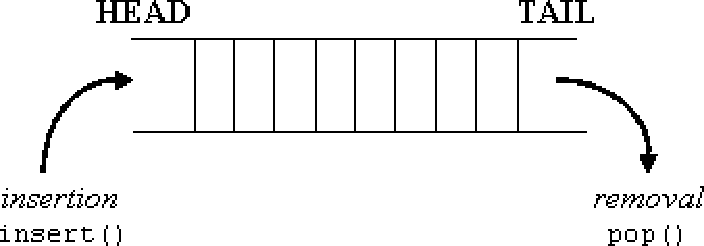
\includegraphics[width=3.703in, height=1.303in]{figures/usmanFig10}
    \caption{What is what with cQueue}
    \label{fig:ch-sim-lib:cqueue}
  \end{center}
\end{figure}

The basic \cclass{cQueue} member functions dealing with insertion and removal
are \fname{insert()} and \fname{pop()}. They are used
like this:

\begin{verbatim}
cQueue queue("my-queue");
cMessage *msg;

// insert messages
for (int i=0; i<10; i++)
{
  msg = new cMessage;
  queue.insert( msg );
}

// remove messages
while( ! queue.empty() )
{
  msg = (cMessage *)queue.pop();
  delete msg;
}
\end{verbatim}


The \fname{length()} member function returns the number of items in the
queue, and \fname{empty()} tells whether there's anything in the queue.

There are other functions dealing with insertion and removal.  The
\fname{insertBefore()} and \fname{insertAfter()} functions insert a
new item exactly before and after a specified one, regardless of the
ordering function.

The \fname{tail()} and \fname{head()} functions return pointers to the objects
at the tail and head of the queue, without affecting queue contents.



The \fname{pop()} function can be used to remove items from the
tail of the queue, and the \fname{remove()} function can be
used to remove any item known by its pointer from the queue:


\fname[queue.remove()]{queue.remove( msg );}



\textbf{Priority queue}


By default, \cclass{cQueue} implements a FIFO, but it can also act as
a priority queue, that is, it can keep the inserted objects
ordered\index{queue!order}.  If you want to use this feature, you have
to provide a function that takes two \cclass{cObject} pointers,
compares the two objects and returns -1, 0 or 1 as the result (see the
reference for details).  An example of setting up an ordered
\cclass{cQueue}:

\begin{verbatim}
cQueue sortedqueue("sortedqueue", cObject::cmpbyname, true );
                        // sorted by object name, ascending
\end{verbatim}


If the queue object is set up as an ordered queue, the \fname{insert()}
function uses the ordering function: it searches the queue contents
from the head until it reaches the position where the new item
needs to be inserted, and inserts it there.


\textbf{Iterators}


Normally, you can only access the objects at the head or tail of the
queue. However, if you use an iterator class, \cclass{cQueueIterator},
you can examine each object in the queue\index{queue!iteration}.

The \cclass{cQueueIterator} constructor takes two arguments, the first
is the queue object and the second one specifies the initial position
of the iterator: 0=tail, 1=head. Otherwise it acts as any other
{\opp} iterator class: you can use the ++ and -- operators to advance
it, the () operator to get a pointer to the current item, and the
\fname{end()} member function to examine if you're at the end (or the
beginning) of the queue.


An example:

\begin{verbatim}
for( cQueueIterator iter(queue,1); !iter.end(), iter++)
{
  cMessage *msg = (cMessage *) iter();
  //...
}
\end{verbatim}




\subsection{Expandable array: cArray}

\textbf{Basic usage}


\cclass{cArray} is a container class that holds objects derived from
\cclass{cObject}. \cclass{cArray} stores the pointers of the objects
inserted instead of making copies. \cclass{cArray} works as an array,
but if it gets full, it grows automatically. Internally,
\cclass{cArray} is implemented with an array of pointers; if the array
gets full, it is reallocated.

\cclass{cArray} objects are used in {\opp} to store parameters
attached to messages, and internally, for storing module parameters
and gates.


Creating an array:

\begin{verbatim}
cArray array("array");
\end{verbatim}

Adding an object at the first free index:

\begin{verbatim}
cPar *p = new cPar("par");
int index = array.add( p );
\end{verbatim}


Adding an object at a given index (if the index is occupied,
you'll get an error message):

\begin{verbatim}
cPar *p = new cPar("par");
int index = array.addAt(5,p);
\end{verbatim}


Finding an object in the array:

\begin{verbatim}
int index = array.find(p);
\end{verbatim}

Getting a pointer to an object at a given index:

\begin{verbatim}
cPar *p = (cPar *) array[index];
\end{verbatim}

You can also search the array or get a pointer to an object by
the object's name:

\begin{verbatim}
int index = array.find("par");
Par *p = (cPar *) array["par"];
\end{verbatim}


You can remove an object from the array by calling \fname{remove()}
with the object name, the index position or the object pointer:

\begin{verbatim}
array.remove("par");
array.remove(index);
array.remove( p );
\end{verbatim}


The \fname{remove()} function doesn't deallocate the object, but it
returns the object pointer. If you also want to deallocate it, you can
write:

\begin{verbatim}
delete array.remove( index );
\end{verbatim}

\textbf{Iteration}


\cclass{cArray} has no iterator, but it's easy to loop through all the
indices with an integer variable. The \fname{items()} member function
returns the largest index plus one.

\begin{verbatim}
for (int i=0; i<array.items(); i++)
{
  if (array[i]) // is this position used?
  {
    cObject *obj = array[i];
    ev << obj->name() << endl;
  }
}
\end{verbatim}




\section{Non-object container classes}

There are two container classes to store non-object
items\index{non-object container}: \cclass{cLinkedList} and
\cclass{cBag}.  The first one parallels with \cclass{cQueue}, the
second one with \cclass{cArray}. They can be useful if you have to
deal with C structs or objects that are not derived from
\cclass{cObject}.

See the class library reference for more info about them.





\section{The parameter class: cPar}

\subsection{Basic usage}

\cclass{cPar} is a class that is designed to hold a value. The value
is numeric (long or double) in the first place, but string, pointer
and other types are also supported.

cPar is used in {\opp} in the following places:

\begin{itemize}
  \item{as module parameters}
  \item{as message parameters}
\end{itemize}

There are many ways to set a \cclass{cPar}'s value. One is the set...Value()
member functions:

\begin{verbatim}
cPar pp("pp");
pp.setDoubleValue(1.0);
\end{verbatim}


or by using overloaded operators:

\begin{verbatim}
cPar pp("pp");
pp = 1.0;
\end{verbatim}


For reading its value, it is best to use overloaded type cast
operators:

\begin{verbatim}
double d1 = (double)pp;
// or simply:
double d2 = pp;
\end{verbatim}

Long integers:

\begin{verbatim}
pp = 89363L; // or:
pp.setLongValue( 89363L );
\end{verbatim}

Character string:

\begin{verbatim}
pp = "hi there"; // or:
pp.setStringValue( "hi there" );
\end{verbatim}


The \cclass{cPar} object makes its own copy of the string, so the
original one does not need to be preserved. Short strings (less than
\ensuremath{\sim}20 chars) are handled more efficiently because they
are stored in the object's memory space (and are not dynamically
allocated).

There are several other types \cclass{cPar} can store: such as boolean,
void* pointer; cObject* pointer,  function with constant args;
they will be mentioned in the next section.

For numeric and string types, an input flag\index{input flag} can be
set. In this case, when the object's value is first used, the
parameter value will be searched for in the configuration (ini)
file\index{ini file}; if it is not found there, the user will be given
a chance to enter the value interactively.


Examples:

\begin{verbatim}
cPar inp("inp");
inp.setPrompt("Enter my value:");
inp.setInput( true );   // make it an input parameter
double a = (double)inp; // the user will be prompted HERE
\end{verbatim}




\subsection{Random number generation through cPar}

Setting \cclass{cPar} to call a function with constant arguments can
be used to make \cclass{cPar} return random variables\index{random!variables} of different distributions\index{distribution}:

\begin{verbatim}
cPar rnd("rnd");
rnd.setDoubleValue(intuniform, -10.0, 10.0);// uniform distr.
rnd.setDoubleValue(normal, 100.0, 5.0); // normal distr. (mean,dev)
rnd.setDoubleValue(exponential, 10.0); // exponential distr. (mean)
\end{verbatim}

\fname{intuniform()}, \fname{normal()} etc. are ordinary C functions
taking double arguments and returning double. Each time you read the
value of a \cclass{cPar} containing a function like above, the
function will be called with the given constant arguments (e.g.
normal(100.0,5.0)) and its return value used.


The above functions use number 0 from the several random number
generators. To use another generator, use the genk\_xxx versions
of the random functions:

\begin{verbatim}
rnd.setDoubleValue(genk\_normal, 3, 100.0, 5.0); // uses generator 3
\end{verbatim}

A \cclass{cPar} object can also be set to return a random variable from
a distribution collected by a statistical data collection object:

\begin{verbatim}
cDoubleHistogram hist =....; // the distribution
cPar rnd2("rnd2");
rnd2.setDoubleValue(hist);
\end{verbatim}




\subsection{Storing object and non-object pointers in cPar}

\cclass{cPar} can store pointers to {\opp} objects. You can use both
assignment and the \fname{setObjectValue()} member function:

\begin{verbatim}
cQueue *queue = new cQueue("queue"); // just an example
cPar par1, par2;
par1 = (cObject *) queue;
par2.setObjectValue( queue );
\end{verbatim}

To get the store pointer back, you can use typecast or the \fname{objectValue()}
member function:

\begin{verbatim}
cQueue *q1 = (cQueue *)(cObject *)par1;
cQueue *q2 = (cQueue *)par2.objectValue();
\end{verbatim}


Whether the \cclass{cPar} object will own the other object or not is
controlled by the \fname{takeOwnership()}\index{ownership} member
function, just as with container classes. This is documented in detail
in the class library reference.  By default, \cclass{cPar} will own
the object.

\cclass{cPar} can be used to store non-object
pointers\index{non-object pointers} (for example C structs) or
non-{\opp} object types in the parameter object.  It works very
similarly to the above mechanism. An example:

\begin{verbatim}
double *mem = new double[15];
cPar par1, par2;
par1 = (void *) mem;
par2.setPointerValue( (void *)mem );
...
double *m1 = (double *)(void *)par1;
double *m2 = (double *)par2.pointerValue();
\end{verbatim}


Memory management\index{cPar memory management} can be specified by
\cclass{cPar}'s \fname{configPointer()} member function. It takes
three arguments: a pointer to a user-supplied deallocation
function, a pointer to a user-supplied duplication function and
an item size. If all three are 0 (NULL), no memory management is done,
that is, the pointer is treated as a mere pointer. This is the default
behaviour. If you supply only the item size (and both function
pointers are NULL), \cclass{cPar} will use the delete operator to
deallocate the memory area when the \cclass{cPar} object is
destructed, and it will use new char[size] followed by a
\fname{memcpy()} to duplicate the memory area whenever the
\cclass{cPar} object is duplicated. If you need more sophisticated
memory management, you can supply your own deallocation and
duplication functions.  All this is documented in detail in the class
library reference.  An example for simple memory management:

\begin{verbatim}
double *mem = new double[15];
cPar par;
par.setPointerValue((void *) mem);
par.configPointer(NULL, NULL, 15*sizeof(double));
// -> now if par goes out of scope, it will delete the 15-double array.
\end{verbatim}

The \fname{configPointer()} setting only affects what happens when the
\cclass{cPar} is deleted, duplicated or copied, but does \textit{not}
apply to assigning new pointers. That is, if \textit{you} assign a new
void* to the \cclass{cPar}, you simply overwrite the pointer -- the
block denoted by the old pointer is \textit{not} deleted. This fact
can be used to extract some dynamically allocated block out of the
\cclass{cPar}: carrying on the previous example, you would extract the
array of 15 doubles from the \cclass{cPar} like this:

\begin{verbatim}
double *mem2 = (double *)par.pointerValue();
par.setValue( (void *)0 );
// -> now par has nothing to do with the double[15] array
\end{verbatim}



However, if you assign some non-pointer value\index{non-pointer value}
to the \cclass{cPar}, beware: this \textit{will} activate the memory
management for the block. If you temporarily use the same
\cclass{cPar} object to store other than void* ('P') values, the
\fname{configPointer()} setting is lost.



\subsection{Reverse Polish expressions}

This feature is rarely needed by the user, it is more used internally.
A \cclass{cPar} object can also store
expressions\index{cPar!expressions}. In this case, the expression must
be given in reversed Polish form\index{reversed polish notation}. An
example:

\begin{verbatim}
sXElem *expression = new sXElem[5];
expression[0] = &par( ''count'' ); // pointer to
module parameter
expression[1] = 1;
expression[2] = '+';
expression[3] = 2;
expression[4] = '/';

cPar expr("expr");
expr.setDoubleValue(expression,5);
\end{verbatim}


The \cclass{cPar} object created above contains the $(count+1)/2$
expression where \textit{count} is a module parameter. Each time the
\cclass{cPar} is evaluated, it recalculates the expression, using the
current value of count. Note the \& sign in front of
\texttt{par(''count'')} expression: if it was not there, the parameter
would be taken by value\index{parameter!by value}, evaluated once and
then the resulting constant would be used.

Another example is a distribution\index{distribution} with mean and
standard deviation given by module parameters:

\begin{verbatim}
sXElem *expression = new sXElem[3];
expression[0] = &par("mean");
expression[1] = &par("stddev");
expression[2] = normal; // pointer to the normal(double,double) func.

cPar expr("expr");
expr.setDoubleValue(expression,3);
\end{verbatim}


For more information, see the reference and the code NEDC generates
for parameter expressions\index{parameter!expressions}.



\subsection{Using redirection}

A \cclass{cPar} object can be set to stand for a value actually stored
in another \cclass{cPar} object. This is called \textit{indirect} or
\textit{redirected} value. When using redirection\index{redirection},
every operation on the value (i.e.  reading or changing it) will be
actually done to the other \cclass{cPar} object:

\begin{figure}[htbp]
  \begin{center}
    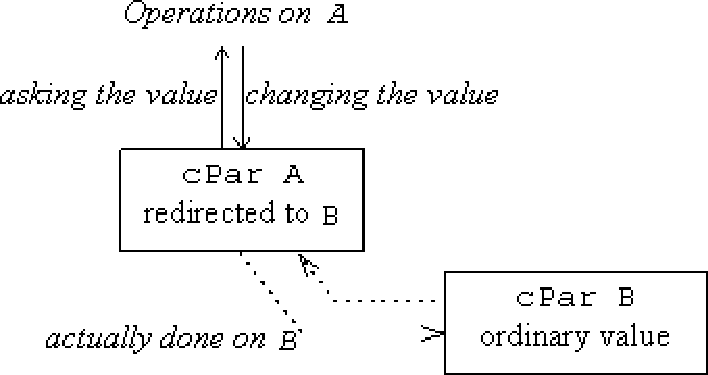
\includegraphics[width=3.608in, height=1.908in]{figures/usmanFig11}
    \caption{cPar redirection}
    \label{fig:ch-sim-lib:cPar-redirection}
  \end{center}
\end{figure}

Redirection is how module parameters taken by
reference\index{module!parameters!by reference} are implemented.  The
redirection does not include name strings. That is, if you say
A-\texttt{>}setName(''newname'') in the above example, A's name will
be changed as the name member is not redirected. (This is natural if
you consider parameters taken by reference: a parameter should/can
have different name than the value it refers to.)


You create a redirection with the \fname{setRedirection()} function:

\begin{verbatim}
cPar *bb = new cPar("bb"); // background value
bb = 10L;
cPar a("a"); // we'll redirect this object

a.setRedirection(bb); // create redirection
\end{verbatim}


Now every operation you do on a's value will be done to bb:

\begin{verbatim}
long x = a; // returns bb's value, 10L
a = 5;      // bb's value changes to 5
\end{verbatim}


The only way to determine whether a is really holding the value or it
is redirected to another \cclass{cPar} is to use the
\fname{isRedirected()} member function which returns a bool, or
\fname{redirection()} which returns the pointer to the background
object, or NULL if there's no redirection:

\begin{verbatim}
cPar *redir = a.redirection(); // returns bb's pointer
if (redir != NULL)
  ev << "a is redirected to " << redir->name() << endl;
\end{verbatim}


To break the link between the two objects, use the
\fname{cancelRedirection()} member function. (No other method will
work, including assigning a the value of another \cclass{cPar}
object.) The \fname{cancelRedirection()} function gives the \texttt{(long)0}
value to the redirected object (the other will be unaffected). If you
want to cancel the indirection but keep the old value, you can do
something like this:

\begin{verbatim}
cPar *value = a.redirection();  // bb's pointer
a.cancelRedirection();          // break the link; value of a is now 0
a = *value;                     // copy the contents of bb into a
\end{verbatim}




\subsection{Type characters}

Internally, \cclass{cPar} objects identify the types of the stored values
by type characters. The type character\index{type character} is returned by the \fname{type()}
member function:

\begin{verbatim}
cPar par = 10L;
char typechar = par.type(); // returns 'L'
\end{verbatim}

The full table of type characters is presented in the \textit{Summary}
section below.

The \fname{isNumeric()} function tells whether the object
stores one of the numeric types, so that e.g. \fname{asDoubleValue()}
can be invoked on it.




\subsection{Summary}

The various \cclass{cPar} types and the member functions\index{cPar
  types and member functions} used to manipulate them are summarized
in the following table:

\begin{longtable}{|p{0.7cm}|p{1.2cm}|p{5.2cm}|p{6cm}|}
\hline
% ROW 1
\tabheadcol
\textbf{Type\linebreak
char} &
\textbf{Type \linebreak
name} &
\textbf{Member functions} &
\textbf{Description}\\
\hline
%% ROW 2
S &  string &
\ttt{setStringValue( \linebreak
\hspace*{0.3cm}  const char *); \linebreak
const char * \linebreak
\hspace*{0.3cm} \fname{stringValue()}; \linebreak
op const char *(); \linebreak
op=(const char *);} &
{\raggedright
string value. Short strings (len\texttt{<}=27) are stored inside
\cclass{cPar} object, without using heap allocation.}\\\hline
%% ROW 3
B &  boolean &
\ttt{setBoolValue(bool); \linebreak
bool \fname{boolValue()}; \linebreak
op \fname{bool()}; \linebreak
op=(bool);} &
boolean value. Can also be retrieved from the object as long  (0 or 1).\\\hline
%% ROW 4
L & long int &
\ttt{setLongValue(long); \linebreak
long \fname{longValue()}; \linebreak
op \fname{long()}; \linebreak
op=(long);} &
signed long integer value. Can also be retrieved from the object
as double.\\\hline
%% ROW 5
D & double &
\ttt{setDoubleValue(double); \linebreak
double \fname{doubleValue()}; \linebreak
op \fname{double()}; \linebreak
op=(double);} &
double-precision floating point value.\\\hline
%% ROW 6
F & function &
\ttt{setDoubleValue( \linebreak
\hspace*{0.3cm} MathFunc, \linebreak
\hspace*{0.3cm} [double], \linebreak
\hspace*{0.3cm} [double], \linebreak
\hspace*{0.3cm} [double]); \linebreak
double \fname{doubleValue()}; \linebreak
op \fname{double()}; \linebreak
} &
Mathematical function with constant arguments. The function
is given by its pointer; it must take 0,1,2 or 3 doubles and
return a double. This type is mainly used to generate random
numbers: e.g. the function takes mean and standard deviation
and returns random variable of a certain distribution.\\\hline
%% ROW 7
X & expr. &
\ttt{setDoubleValue( \linebreak
\hspace*{0.3cm} sXElem*,int); \linebreak
double \fname{doubleValue()}; \linebreak
op \fname{double()};}
&
Reverse Polish expression. Expression can contain constants,
\cclass{cPar} objects, refer to other \cclass{cPars} (e.g. module parameters),
can use many math operators (+-*/{\textasciicircum}\% etc), function calls
(function must take 0,1,2 or 3 doubles and return a double).
The expression must be given is in an sXElem array (see later).\\\hline
%% ROW 8
T & distrib. &
\ttt{setDoubleValue( \linebreak
\hspace*{0.3cm} \cclass{cStatistic}*); \linebreak
double \fname{doubleValue()}; \linebreak
op \fname{double()}; \linebreak
} &
random variable generated from a distribution collected by a
statistical data collection object (derived from \cclass{cStatistic}).\\\hline
%% ROW 9
P & void* pointer &
\ttt{setPointerValue(void*); \linebreak
void *\fname{pointerValue()}; \linebreak
op void *(); \linebreak
op=(void *);} &
pointer to a non-\cclass{cObject} item (C struct, non-\cclass{cObject} object
etc.) Memory management can be controlled through the \fname{configPointer()}
member function.\\\hline
%% ROW 10
O & object pointer &
\ttt{setObjectValue(cObject*); \linebreak
cObject *\fname{objectValue()}; \linebreak
op cObject *(); \linebreak
op=(cObject *);}
&
{\raggedright pointer to an object derived from \cclass{cObject}.\\
Ownership management is done through \fname{takeOwnership()}.}\\\hline
%% ROW 11
I & indirect value &
\ttt{setRedirection(cPar*); \linebreak
bool \fname{isRedirected()}; \linebreak
cPar *\fname{redirection()}; \linebreak
\fname{cancelRedirection()};}
&
{\raggedright value is redirected to another \cclass{cPar} object. All value setting
and reading operates on the other \cclass{cPar}; even the \fname{type()} function
will return the type in the other \cclass{cPar} (so you'll never get 'I'
as the type). This redirection can only be broken with the \fname{cancelRedirection()}
member function.\\
Module parameters taken by REF use this mechanism.}\\\hline
\end{longtable}







\section{Statistics and distribution estimation}

\subsection{
cStatistic and descendants}

There are several statistic and result collection classes:
\cclass{cStdDev}, \cclass{cWeightedStdDev}, \cclass{Long\-Histogram},
\cclass{cDoubleHistogram}, \cclass{cVarHistogram}, \cclass{cPSquare} and
\cclass{cKSplit}. They are all derived from the abstract base class
\cclass{cStatistic}.

\begin{itemize}
  \item{\cclass{cStdDev} keeps number of samples, mean, standard
    deviation, minimum and maximum value etc.}
  \item{\cclass{cWeightedStdDev} is similar to \cclass{cStdDev}, but
    accepts weighted observations. \cclass{cWeightedStdDev} can be used
    for example to calculate time average. It is the only weighted
    statistics class.}
  \item{\cclass{cLongHistogram} and \cclass{cDoubleHistogram} are
    descendants of \cclass{cStdDev} and also keep an approximation of
    the distribution of the observations using equidistant
    (equal-sized) cell histograms\index{histogram!equal-sized}.}
  \item{\cclass{cVarHistogram} implements a histogram where cells do not
    need to be the same size. You can manually add the cell (bin)
    boundaries, or alternatively, automatically have a partitioning
    created where each bin has the same number of observations (or as
    close to that as possible).}
  \item{\cclass{cPSquare} is a class that uses the $P^{2}$ algorithm
    described in [JCH85]. The algorithm calculates quantiles without
    storing the observations; one can also think of it as a histogram
    with equiprobable cells\index{histogram!equiprobable-cells}.}
  \item{\cclass{cKSplit} uses a novel, experimental method, based on an
    adaptive histogram-like algorithm. (Published papers about
    \textit{k-split}\index{k-split} can be downloaded from the {\opp}
    Web site; just go one level up in the directories:
    http://www.hit.bme.hu/phd/vargaa). Because k-split is not very
    well known, we'll devote a section to it.}
\end{itemize}

\textbf{Basic usage}


One can insert an observation into a statistic object with the
\fname{collect()} function or the \texttt{+=} operator (they are
equivalent).  \cclass{cStdDev} has the following methods for getting
statistics out of the object: \fname{samples()}, \fname{min()},
\fname{max()}, \fname{mean()}, \fname{stddev()}, \fname{variance()},
\fname{sum()}, \fname{sqrSum()} with the obvious meanings. An example
usage for \cclass{cStdDev}:

\begin{verbatim}
cStdDev stat("stat");
for (int i=0; i<10; i++)
  stat.collect( normal(0,1) );
long num_samples = stat.samples();
double smallest = stat.min(),
largest = stat.max();
double mean = stat.mean(),
standard_deviation = stat.stddev(),
variance = stat.variance();
\end{verbatim}






\subsection{Distribution estimation}

\textbf{Initialization and usage}


The distribution estimation\index{distribution!estimation} classes (the histogram classes,
\cclass{cPSquare} and \cclass{cKSplit}) are derived from
\cclass{cDensityEstBase}. Distribution estimation classes (except for
\cclass{cPSquare}) assume that the observations are within a range.
You may specify the range explicitly (based on some a-priori info
about the distribution) or you may let the object collect the first
few observations and determine the range from them. Methods which let
you specify range settings are part of \cclass{cDensityEstBase}. The
following member functions exist:

\begin{verbatim}
setRange(lower,upper);
setRangeAuto(num_firstvals, range_ext_factor);
setRangeAutoLower(upper, num_firstvals, range_ext_factor);
setRangeAutoUpper(lower, num, range_ext_factor);
\end{verbatim}

\textbf{setNumFirstVals(num\_firstvals);}


The following example creates a histogram with 20 cells and automatic
range estimation\index{histogram!range estimation}:

\begin{verbatim}
cDoubleHistogram histogram("histogram", 20);
histogram.setRangeAuto(100,1.5);
\end{verbatim}


Here, 20 is the number of cells (not including the underflow/overflow
cells, see later), and 100 is the number of observations to be
collected before setting up the cells. 1.5 is the range extension
factor. It means that the actual range of the initial observations
will be expanded 1.5 times and this expanded range will be used to lay
out the cells. This method increases the chance that further
observations fall in one of the cells and not outside the histogram
range.

\begin{figure}[htbp]
  \begin{center}
    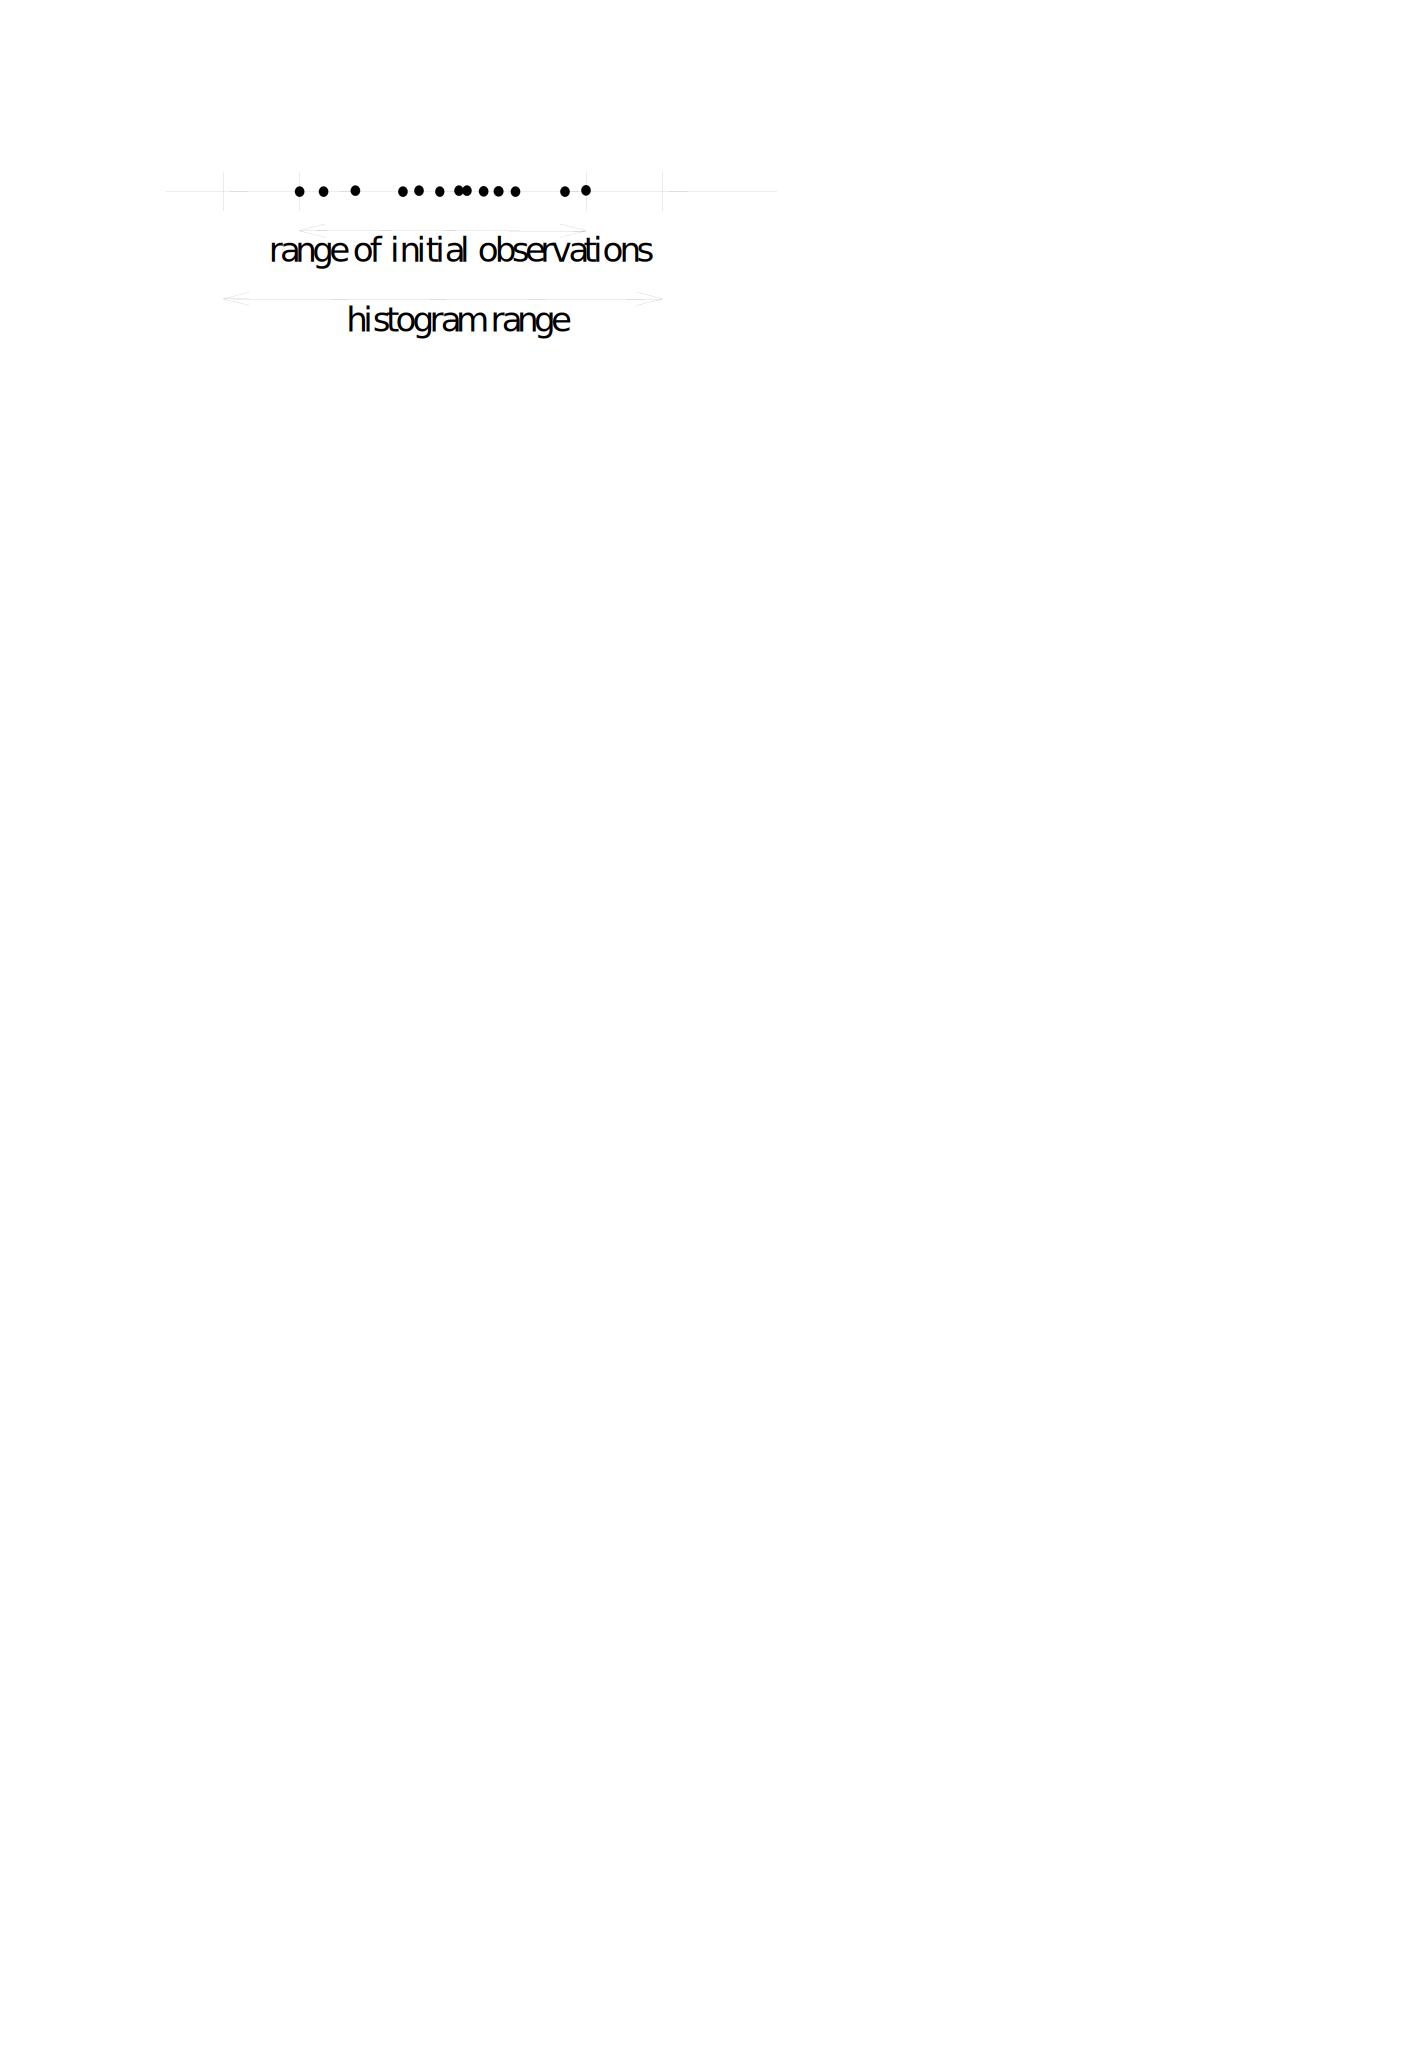
\includegraphics[width=3.215in, height=0.930in]{figures/usmanFig12}
    \caption{Setting up a histogram's range}
  \end{center}
\end{figure}

After the cells have been set up, collecting can go on.

The \fname{transformed()} function returns \textit{true} when the cells have
already been set up. You can force range estimation and setting
up the cells by calling the \fname{transform()} function.

The observations that fall outside the histogram range will be counted
as underflows and overflows. The number of underflows and overflows
are returned by the \fname{underflowCell()} and \fname{overflowCell()}
member functions.

\begin{figure}[htbp]
\begin{center}
  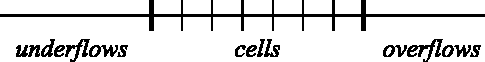
\includegraphics[width=3.310in, height=0.467in]{figures/usmanFig13}
  \caption{Histogram structure after setting up the cells}
\end{center}
\end{figure}

You create a $P^{2}$ object by specifying the number of cells:

\begin{verbatim}
cPSquare psquare("interarrival-times", 20);
\end{verbatim}

Afterwards, a \cclass{cPSquare} can be used with the same member functions
as a histogram.


\textbf{Getting histogram data}


There are three member functions to explicitly return cell boundaries
and the number of observations is each cell. \fname{cells()} returns
the number of cells, \fname[basepoint()]{basepoint(int k)} returns the
\textit{k}th base point, \fname[cell()]{cell(int k)} returns the
number of observations in cell \textit{k}, and
\fname[cellPDF()]{cellPDF(int k)} returns the PDF value in the cell
(i.e. between \fname[basepoint()]{basepoint(k)} and
\fname[basepoint()]{basepoint(k+1)}).  These functions work for all
histogram types, plus \cclass{cPSquare} and \cclass{cKSplit}.

\begin{figure}[htbp]
  \begin{center}
    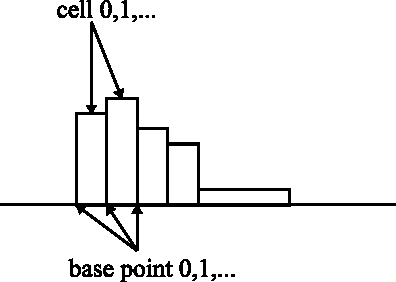
\includegraphics[width=2.615in, height=2.001in]{figures/usmanFig14}
    \caption{base points and cells}
  \end{center}
\end{figure}

An example:

\begin{verbatim}
long n = histogram.samples();
for (int i=0; i<histogram.cells(); i++)
{
  double cellWidth = histogram.basepoint(i+1)-histogram.basepoint(i);
  int count = histogram.cell(i);
  double pdf = histogram.cellPDF(i);
  //...
}
\end{verbatim}


The \fname[pdf()]{pdf(x)} and \fname[cdf()]{cdf(x)} member functions
return the value of the probability density function and the cumulated
density function at a given \textit{x}, respectively.


\textbf{Random number generation from distributions}


The \fname{random()} member function generates random
numbers\index{random!numbers} from the distribution stored by the
object:

\begin{verbatim}
double rnd = histogram.random();
\end{verbatim}


\cclass{cStdDev} assumes normal distribution.

You can also wrap the distribution object in a \cclass{cPar}:

\begin{verbatim}
cPar rnd_par("rnd_par");
rnd_par.setDoubleValue(&histogram);
\end{verbatim}


The \cclass{cPar} object stores the pointer to the histogram (or $P^{2}$ object),
and whenever it is asked for the value, calls the histogram object's \fname{random()}
function:

\begin{verbatim}
double rnd = (double)rnd_par; // random number from the cPSquare
\end{verbatim}

\textbf{Storing/loading distributions}


The statistic classes have \fname{loadFromFile()} member functions
that read the histogram data from a text file. If you need a custom
distribution\index{distribution!custom} that cannot be written (or it
is inefficient) as a C function, you can describe it in histogram form
stored in a text file, and use a histogram object with
\fname{loadFromFile()}.

You can also use \fname{saveToFile()}that writes out the distribution
collected by the histogram object:

\begin{verbatim}
FILE *f = fopen("histogram.dat","w");
histogram.saveToFile( f ); // save the distribution
fclose( f );

FILE *f2 = fopen("histogram.dat","r");}
cDoubleHistogram hist2("Hist-from-file");
hist2.loadFromFile( f2 ); // load stored distribution
fclose( f2 );
\end{verbatim}


\textbf{Histogram with custom cells}


The \cclass{cVarHistogram} class can be used to create
histograms with arbitrary (non-equidistant) cells.
It can operate in two modes:

\begin{itemize}
  \item \textit{manual}, where you specify cell boundaries explicitly
     before starting collecting
  \item \textit{automatic}, where \fname{transform()} will set up the cells
     after collecting a certain number of initial observations. The cells
     will be set up so that as far as possible, an equal number of observations
     fall into each cell (equi-probable cells).
\end{itemize}

Modes are selected with a \textit{transform-type} parameter:
\begin{itemize}
  \item{\ttt{HIST\_TR\_NO\_TRANSFORM}: no transformation; uses bin boundaries
    previously defined by \fname{addBinBound()}}
  \item{\ttt{HIST\_TR\_AUTO\_EPC\_DBL}: automatically creates equiprobable cells}
  \item{\ttt{HIST\_TR\_AUTO\_EPC\_INT}: like the above, but for integers}
\end{itemize}

Creating an object:

\begin{verbatim}
cVarHistogram(const char *s=NULL,
              int numcells=11,
              int transformtype=HIST_TR_AUTO_EPC_DBL);
\end{verbatim}

Manually adding a cell boundary:

\begin{verbatim}
void addBinBound(double x);
\end{verbatim}

Rangemin and rangemax is chosen after collecting the
\texttt{num\_firstvals} initial observations. One cannot add cell
boundaries when the histogram has already been transformed.





\subsection{The k-split algorithm}

\textbf{Purpose}


The \textit{k}-split algorithm is an on-line distribution
estimation\index{distribution!online estimation} method.  It was
designed for on-line result collection in simulation programs.  The
method was proposed by Varga and Fakhamzadeh in 1997. The primary
advantage of \textit{k}-split is that without having to store the
observations, it gives a good estimate without requiring a-priori
information about the distribution, including the sample size. The
\textit{k}-split algorithm can be extended to multi-dimensional
distributions\index{distribution!multi-dimensional}, but here we deal
with the one-dimensional version only.


\textbf{The algorithm}


The \textit{k-split} algorithm is an adaptive histogram-type estimate which
maintains a good partitioning by doing cell splits. We start out with
a histogram range $[x_{lo}, x_{hi})$ with $k$ equal-sized histogram
cells with observation counts $n_1,n_2, \cdots n_k$.  Each collected
observation increments the corresponding observation count. When an
observation count $n_i$ reaches a \textit{split threshold}, the cell
is split into $k$ smaller, equal-sized cells with observation counts
$n_{i,1}, n_{i,2}, \cdots n_{i,k}$ initialized to zero. The $n_i$
observation count is remembered and is called the \textit{mother
  observation count} to the newly created cells. Further observations
may cause cells to be split further (e.g. $n_{i,1,1},...n_{i,1,k}$
etc.), thus creating a $k$-order tree of observation counts where
leaves contain live counters that are actually incremented by new
observations, and intermediate nodes contain mother observation counts
for their children. If an observation falls outside the histogram
range, the range is extended in a natural manner by inserting new
level(s) at the top of the tree. The fundamental parameter to the
algorithm is the split factor $k$. Low values of $k$, $k=2$ and $k=3$
are to be considered. In this paper we examine only the $k=2$ case.

\begin{figure}[htbp]
  \begin{center}
    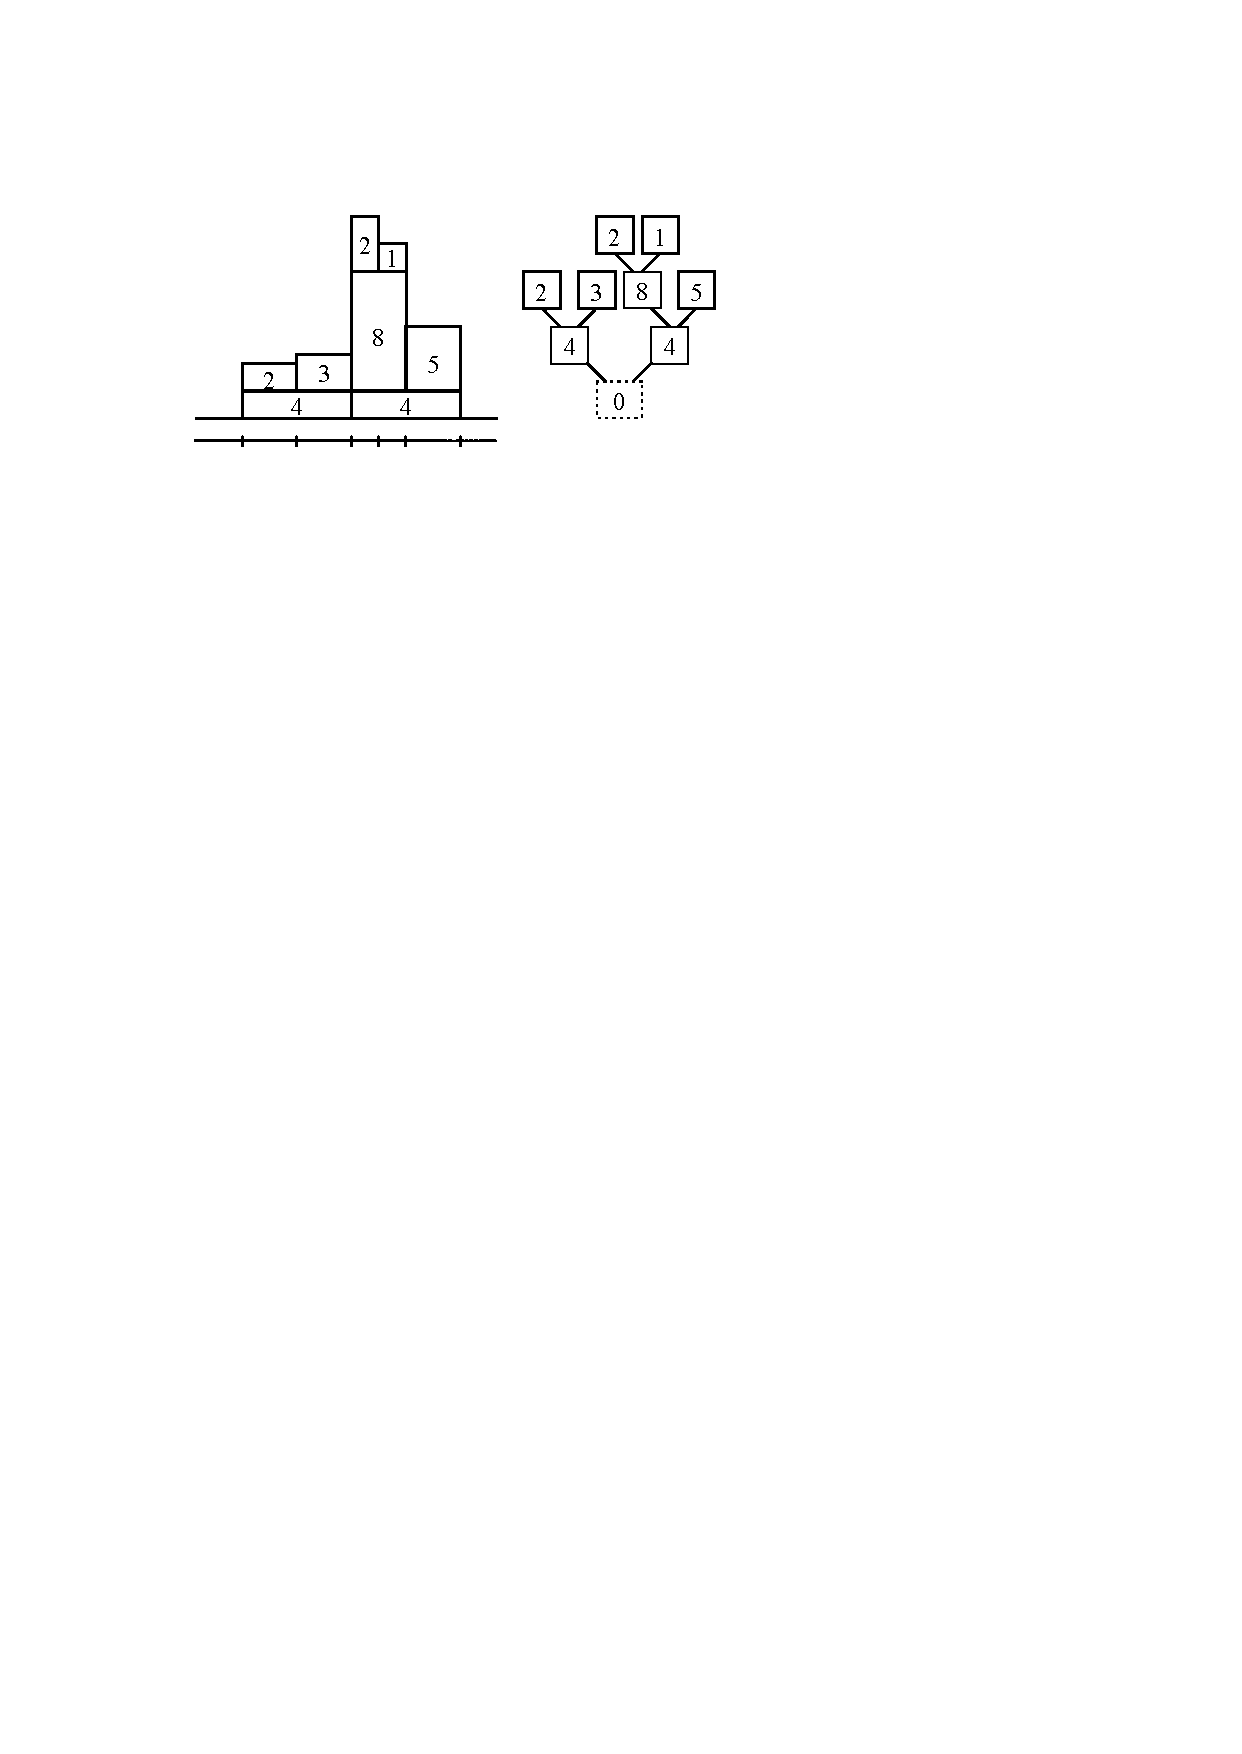
\includegraphics[width=3.442in, height=1.518in]{figures/usmanFig15}
    \caption{Illustration of the k-split algorithm, $k=2$. The
      numbers in boxes represent the observation count values}
  \end{center}
\end{figure}


For density estimation, the total number of observations that
fell into each cell of the partition has to be determined. For
this purpose, mother observations in each internal node of the
tree must be distributed among its child cells and propagated
up to the leaves.


Let $n_{...,i}$ be the (mother) observation count for a cell,
$s_{...,i}$ be the total observation count in a cell $n_{...,i}$ plus
the observation counts in all its sub-, sub-sub-, etc. cells), and
$m_{...,i}$ the mother observations propagated to the cell. We are
interested in the $\tilde{n}_{...,i} = n_{...,i} + m_{...,i}$
estimated amount of observations in the tree nodes, especially in the
leaves. In other words, if we have $\tilde{n}_{...,i}$ estimated
observation amount in a cell, how to divide it to obtain $m_{...,i,1},
m_{...,i,2} \cdots m_{...,i,k}$ that can be propagated to child cells.
Naturally, $m_{...,i,1} + m_{...,i,2} + \cdots + m_{...,i,k} =
\tilde{n}_{...,i}$.


Two natural distribution methods are even
distribution\index{distribution!even} (when $m_{...,i,1} = m_{...,i,2}
= \cdots = m_{...,i,k}$) and proportional
distribution\index{distribution!proportional} (when $m_{...,i,1} :
m_{...,i,2} : \cdots : m_{...,i,k} = s_{...,i,1} : s_{...,i,2} :
\cdots : s_{...,i,k}$). Even distribution is optimal when the
$s_{...,i,j}$ values are very small, and proportional distribution is
good when the $s_{...,i,j}$ values are large compared to
$m_{...,i,j}$. In practice, a linear combination of them seems
appropriate, where $\lambda=0$ means even and $\lambda=1$ means
proportional distribution:


\begin{equation}
m_{\cdots,i,j}=(1-\lambda )\frac{\tilde{n}_{\cdots,i}}{k} + \lambda \tilde{n}_{\cdots,i} \frac{s_{...,i,j}}{s_{\cdots,i}}, {\lambda}\in[0,1]
\end{equation}

\begin{figure}[htbp]
  \begin{center}
    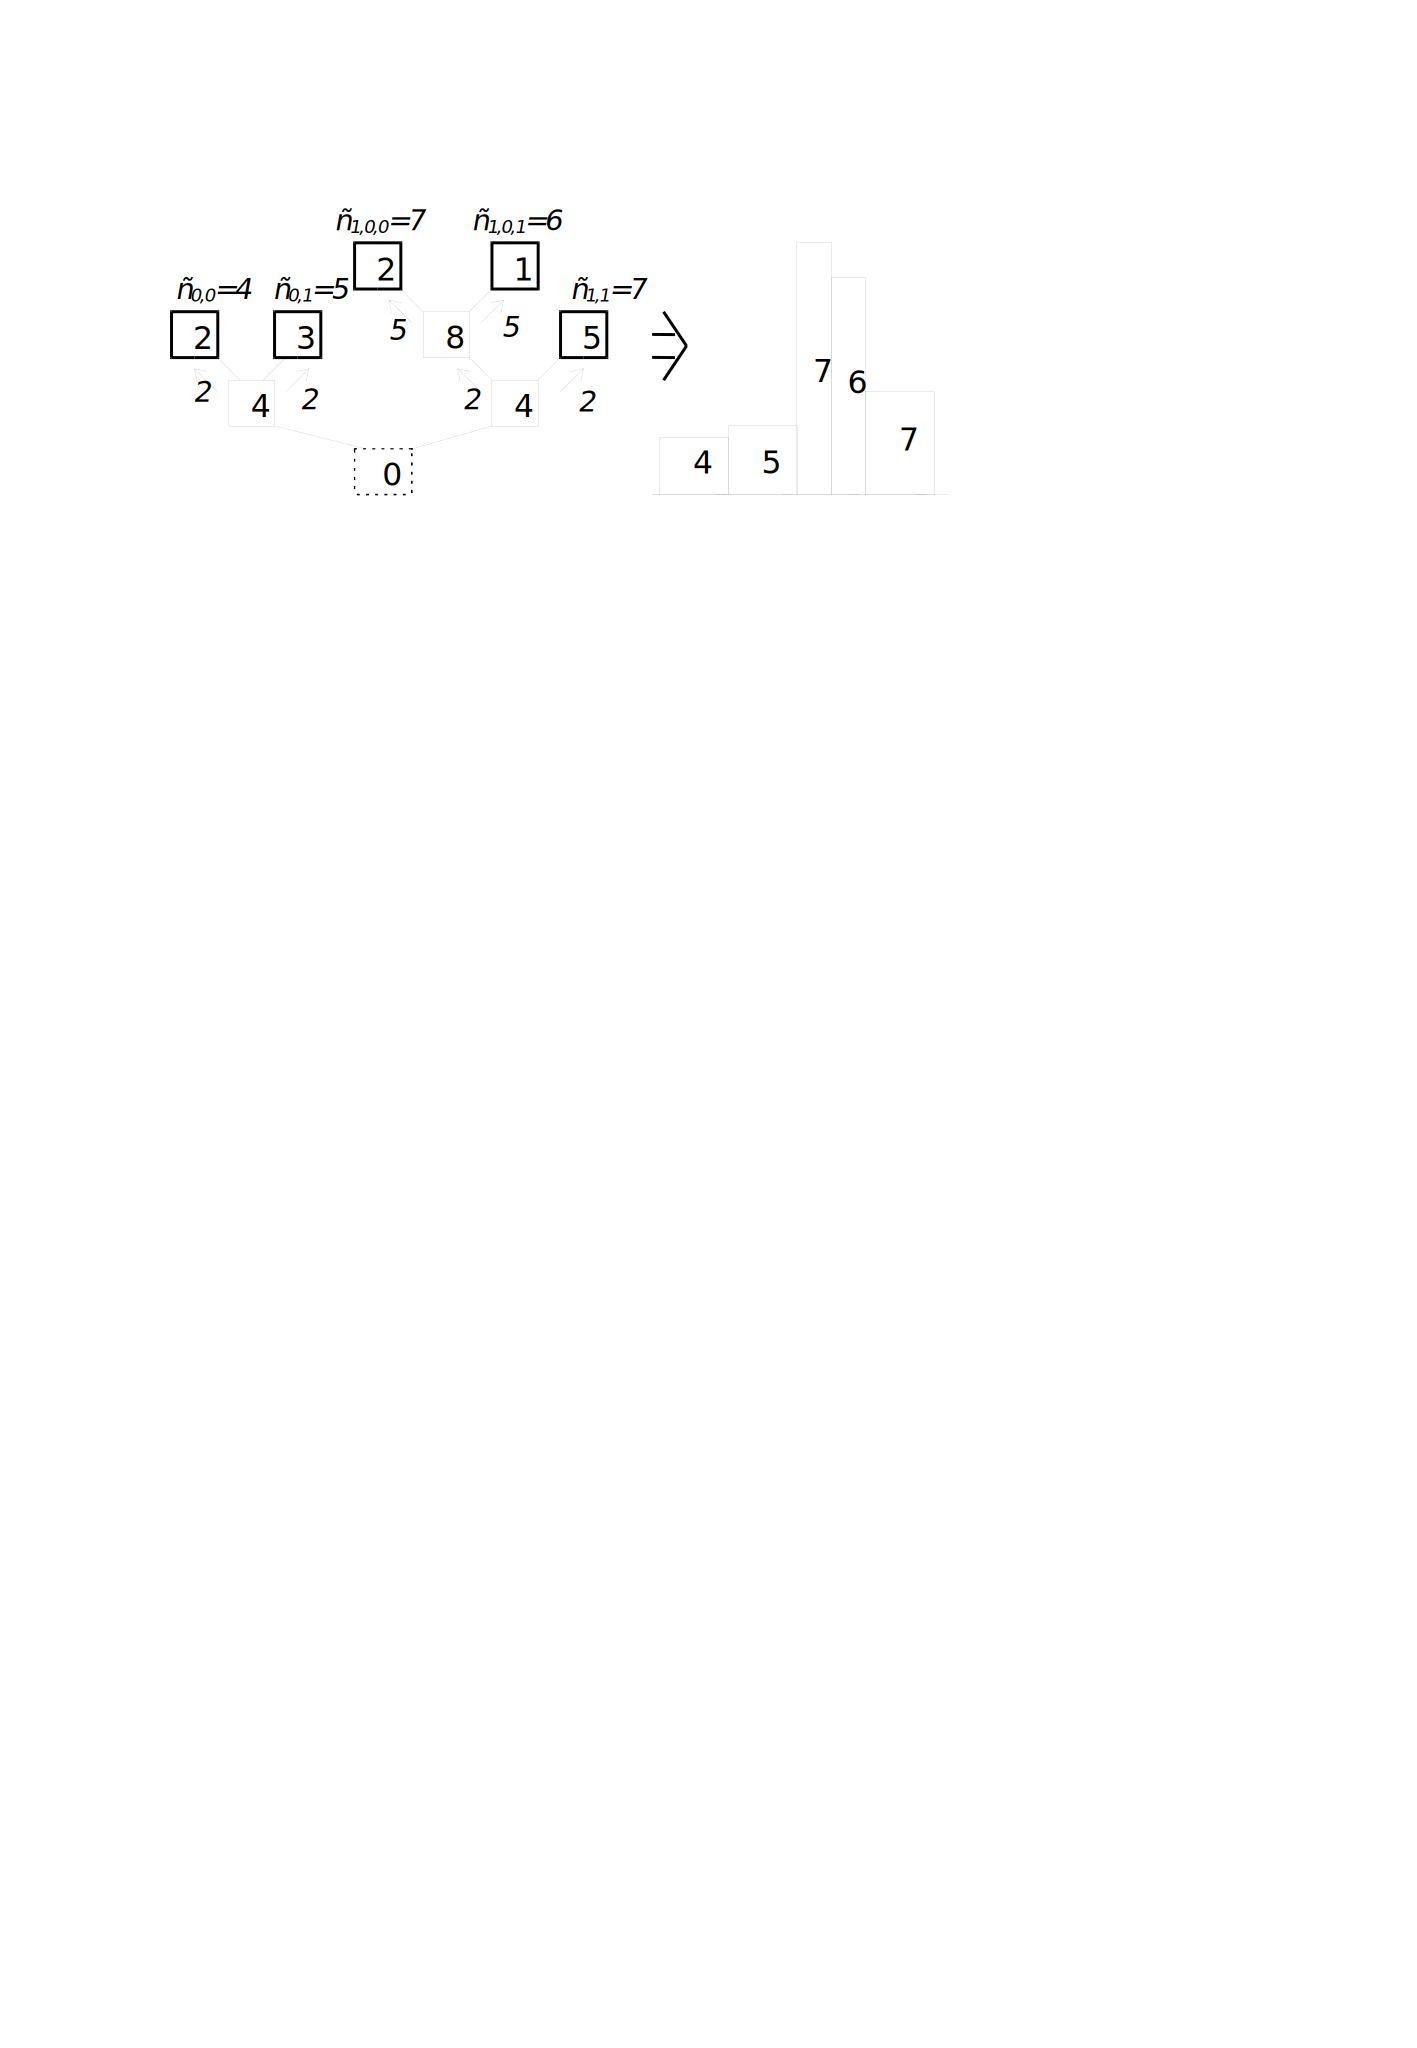
\includegraphics[width=4.147in, height=1.567in]{figures/usmanFig16}
    \caption{Density estimation from the k-split cell tree. We
      assume $\lambda=0$, i.e. we distribute mother observations
      evenly.}
  \end{center}
\end{figure}

Note that while $n_{...,i}$ are integers, $m_{...,i}$ and thus
$\tilde{n}_{...,i}$ are typically real numbers. The histogram estimate
calculated from \textit{k}-split is not exact, because the frequency
counts calculated in the above manner contain a degree of estimation
themselves. This introduces a certain \textit{cell division error};
the $\lambda$ parameter should be selected so that it minimizes that
error. It has been shown that the cell division error can
be reduced to a more-than-acceptable small value.\\
Strictly speaking, the \textit{k}-split algorithm is semi-online,
because its needs some observations to set up the initial histogram
range.  However, because of the range extension and cell split
capabilities, the algorithm is not very sensitive to the choice of the
initial range, so very few observations are enough for range
estimation (say $N_{pre}=10$). Thus we can regard \textit{k}-split as
an on-line method.

\textit{K}-split can also be used in semi-online mode, when the
algorithm is only used to create an optimal partition from a larger
number of $N_{pre}$ observations. When the partition has been created,
the observation counts are cleared and the $N_{pre}$ observations are
fed into \textit{k}-split once again. This way all mother (non-leaf)
observation counts will be zero and the cell division error is
eliminated. It has been shown that the partition created by
\textit{k}-split can be better than both the equi-distant and the
equal-frequency partition.


{\opp} contains an experimental implementation of the \textit{k}-split
algorithm, the \cclass{cKSplit} class. Research on \textit{k}-split is
still under way.


\textbf{The cKSplit class}

The \cclass{cKSplit} class is an implementation of the \textit{k-split} method.
Member functions:

%
% TBD comments
%

\begin{verbatim}
void setCritFunc(KSplitCritFunc _critfunc, double *_critdata);
void setDivFunc(KSplitDivFunc \_divfunc, double *\_divdata);
void rangeExtension( bool enabled );
\end{verbatim}


\begin{verbatim}
int treeDepth();
int treeDepth(sGrid& grid);
\end{verbatim}

\begin{verbatim}
double realCellValue(sGrid& grid, int cell);
void printGrids();
\end{verbatim}

\begin{verbatim}
sGrid& grid(int k);
sGrid& rootGrid();
\end{verbatim}

\begin{verbatim}
struct sGrid
{
  int parent;   // index of parent grid
  int reldepth; // depth = (reldepth - rootgrid's reldepth)
  long total;   // sum of cells & all subgrids (includes 'mother')
  int mother;   // observations 'inherited' from mother cell
  int cells[K]; // cell values
};
\end{verbatim}



\subsection{Transient detection and result accuracy}

In many simulations, only the steady state performance (i.e.
the performance after the system has reached a stable state)
is of interest. The initial part of the simulation is called
the transient period. After the model has entered steady state,
simulation must proceed until enough statistical data have been
collected to compute result with the required accuracy.


Detection of the end of the transient period and a certain result
accuracy is supported by {\opp}. The user can attach transient
detection\index{transient detection} and result accuracy\index{result
  accuracy} objects to a result object (\cclass{cStatistic}'s
descendants). The transient detection and result accuracy objects will
do the specific algorithms on the data fed into the result object and
tell if the transient period is over or the result accuracy has been
reached.

The base classes for classes implementing specific transient
detection and result accuracy detection algorithms are:
\begin{itemize}
\item{\cclass{cTransientDetection}: base class for transient detection}
\item{\cclass{cAccuracyDetection}: base class for result accuracy detection}
\end{itemize}


\textbf{Basic usage}

%
% TBD comments
%

Attaching detection objects to a \cclass{cStatistic} and getting pointers
to the attached objects:

\begin{verbatim}
addTransientDetection(cTransientDetection *object);
addAccuracyDetection(cAccuracyDetection *object);
cTransientDetection *transientDetectionObject();
cAccuracyDetection *accuracyDetectionObject();
\end{verbatim}


Detecting the end of the period:
\begin{itemize}
\item{polling the \fname{detect()} function of the object}
\item{installing a post-detect function}
\end{itemize}


\textbf{Transient detection}


Currently one transient detection\index{transient detection} algorithm
is implemented, i.e.  there's one class derived from
\cclass{cTransientDetection}. The \cclass{cTDExpandingWindows} class
uses the sliding window approach with two windows, and checks the
difference of the two averages to see if the transient period is over.

\begin{verbatim}
void setParameters(int reps=3,
                   int minw=4,
                   double wind=1.3,
                   double acc=0.3);
\end{verbatim}

\textbf{Accuracy detection}


Currently one accuracy detection\index{accuracy detection} algorithm
is implemented, i.e.  there's one class derived from
\cclass{cAccuracyDetection}. The algorithm implemented in the
\cclass{cADByStddev} class is: divide the standard deviation by the
square of the number of values and check if this is small enough.

\begin{verbatim}
void setParameters(double acc=0.1,
                   int reps=3);
\end{verbatim}




\section{Recording simulation results}

\subsection{Output vectors: cOutVector}

Objects of type \cclass{cOutVector} are responsible for writing time series
data (referred to as \textit{output vectors}) to a file. The \fname{record()}
member is used to output a value (or a value pair) with a timestamp.

It can be used like this:

\begin{verbatim}
cOutVector resp_v("response time");

while (...)
{
  double response_time;
  //...
  resp_v.record( response_time );
  //...
}
\end{verbatim}


All \cclass{cOutVector} objects write to the same, common file. The
file is textual; each \fname{record()} call generates a line in the
file. The output file can be processed using Plove, but otherwise its
simple format allows it to be easily processed with \fprog{sed},
\fprog{awk}, \fprog{grep} and the like, and it can be imported by
spreadsheet programs.  The file format is described later in this
manual (in the section about simulation execution).

You can disable the output vector\index{output!vector} or specify a
simulation time interval for recording either from the ini file or
directly from program code:

\begin{verbatim}
cOutVector v("v");
simtime_t t =...;

v.enable();
v.disable();
v.setStartTime( t );
v.setStopTime( t+100.0 );
\end{verbatim}


If the output vector object is disabled or the simulation time is
outside the specified interval, \fname{record()} doesn't write
anything to the output file. However, if you have a Tkenv inspector
window open for the output vector object\index{output!vector object},
the values will be displayed there, regardless of the state of the
output vector object.





\subsection{Output scalars}

While output vectors are to record time series data and thus they
typically record a large volume of data during a simulation run,
output scalars\index{output!scalars} are supposed to record a single
value per simulation run. You can use outputs scalars
\begin{itemize}
\item{to record summary data at the end of the simulation run}
\item{to do several runs with different parameter settings/random seed
    and determine the dependence of some measures on the parameter
    settings. For example, multiple runs and output scalars are the
    way to produce \textit{Throughput vs. Offered Load} plots.}
\end{itemize}

Output scalars are recorded with the \fname{recordScalar()} member
function.  It is overloaded, you can use it to write doubles and
strings (const char *):

\begin{verbatim}
double avg_throughput = total_bits / simTime();
recordScalar("Average throughput", avg_throughput);
\end{verbatim}


You can record whole statistics objects by calling \fname{recordStats()}:

\begin{verbatim}
cStdDev *eedstats = new cStdDev;
...
recordStats("End-to-end Statistics", eedstats);
\end{verbatim}



Calls to \fname{recordScalar()} and \fname{recordStats()} are usually
placed in the redefined \fname{finish()} member function of a
simple module.


The above calls write into the (textual) output scalar file.  The
output scalar file is preserved across simulation runs (unlike the
output vector file is, scalar files are not deleted at the beginning
of each run). Data are always appended at the end of the file, and
output from different simulation runs are separated by special lines.





\section{Deriving new classes}

Nearly all classes in the simulation class library are descendants of
\cclass{cObject}. If you want to derive a new class from
\cclass{cObject} or a \cclass{cObject} descendant, you must redefine
some member functions so that objects of the new type can fully
co-operate with other parts of the simulation system. A more-or-less
complete list of these functions are presented here. Do not be
embarrassed at the length of the list: most functions are not
absolutely necessary to implement. For example, you do not need to
redefine \fname{forEach()} unless your class is a container class.

\begin{itemize}
  \item{default constructor, copy constructor. The copy constructor
    can simply call the assignment operator.}
  \item{\fname{operator=()}: the assignment operator (copies object
    contents from another object)}
  \item{\fname{dup()}: duplicates the object by creating an exact copy
    (uses copy constructor\index{copy constructor})}
  \item{\fname{info()}: returns a one-line info about object contents}
  \item{\fname{writeContents()}: write a more detailed report about the
    object into a file}
  \item{\fname{forEach()}: iterates through all contained objects if
    any}
  \item{\fname{netPack()}, \fname{netUnpack()}: they are needed only if
    objects of this type will be sent over
    PVM\index{PVM}/MPI\index{MPI} from one segment to another.  The
    \fname{netPack()},\fname{netUnpack()}functions of the library
    classes are in the sim/pvm (sim/mpi) directory.}
\end{itemize}

One should also use the \fmac{Register\_Class()} macro to register the
new class. It is used by the \fname{createOne()} function and the
PVM/MPI extension of {\opp}.

Let us see a simple example. The header file:

\begin{verbatim}
// File: cmyclass.h
#include <omnetpp.h>

class cMyClass : public cObject
{
 public:
  int samples;

  cMyClass(const cMyClass& myclass);
  cMyClass(const char *name=NULL, int k=0);
  virtual ~cMyClass() {}
  virtual cObject *dup() const {return new cMyClass(*this);}
  virtual void info(char *buf);
  virtual void writeContents(ostream& os);
  cMyClass& operator=(const cMyClass& myclass);
};
\end{verbatim}

The corresponding .cc file:

\begin{verbatim}
// File: cmyclass.cc
#include <stdio.h>
#include <string.h>
#include <iostream.h>
#include "cmyclass.h"

Register_Class( cMyClass );

cMyClass::cMyClass(const cMyClass& myclass) : cObject()
{
  setName( myclass.name() );
  operator=( myclass );
}

cMyClass::cMyClass(const char *name, int k) : cObject( name )
{
  samples = k;
}

void cMyClass::info(char *buf)
{
  cObject::info( buf );
  sprintf( buf+strlen(buf), " samples=%d", samples);
}

void cMyClass::writeContents(ostream& os)
{
  os << " samples: " << samples << '\n';
}

cMyClass& cMyClass::operator=(const cMyClass& myclass)
{
  cObject::operator=(myclass);
  samples = myclass.samples;
}
\end{verbatim}


See the virtual functions of \cclass{cObject} in the class library reference
for more information.





\section{Tracing and debugging aids}

\subsection{Displaying information about module activity}

You can have simple modules print textual output for
debugging\index{debugging} purposes.

The global object called ev represents the user interface of the
simulation program. You can send data to ev\index{ev} using the
C++-style I/O operator (\ttt{<}\ttt{<}).

\begin{verbatim}
ev << "started\n";
ev << "about to send message #" <<  i << endl;
ev << "queue full, discarding packet\n";
\end{verbatim}

The more traditional-looking but functionally equivalent
\fname{ev.printf()} form also exists.

\begin{verbatim}
ev.printf("%d packets dropped out of %d\n", drops, total);
\end{verbatim}

The exact way messages are displayed to the user depends on the user
interface. In the command-line user interface (Cmdenv\index{Cmdenv}),
it is simply dumped to the standard output. (This output can also be
disabled from the ini file so that it doesn't slow down simulation
when it is not needed.) In windowing user interfaces
(Tkenv\index{Tkenv}), each simple module can have
a separate text output window.

The above means that you should \textit{not} use \fname{printf()},
\fname{cout} \fname{<<} and the like because with Tkenv, their output
would appear in the terminal window behind the graphical window of the
simulation application.


\subsection{Watches}

You may want some of your int, long, double, char, etc. variables to
be inspect-able in Tkenv and to be output into the snapshot
file\index{snapshot file}. In this case, you can create
\cclass{cWatch} objects for them with the \fmac{WATCH()} macro:

\begin{verbatim}
int i; WATCH(i);
char c; WATCH(c);
\end{verbatim}

When you open an inspector for the simple module in Tkenv and click
the Objects/Watches tab in it, you'll see your WATCHed variables
and their values there. Tkenv also lets you change the value of a
WATCHed variable.

The \fmac{WATCH()} macro expands to a dynamically created \cclass{cWatch}
object.  The object remembers the address and type of your variable.
The macro expands to something like:

\begin{verbatim}
new cWatch("i",i);
\end{verbatim}


You can also make a \texttt{WATCH} for pointers of type \ttt{char*} or
\cclass[cObject]{cObject*}, but this may cause a segmentation fault if
the pointer does not point to a valid location when Tkenv or
\fname{snapshot()} wants to use it.

You can also set watches for variables that are members of the
module class\index{module!watches} or for structure fields:

\begin{verbatim}
WATCH( lapbconfig.timeout );
\end{verbatim}


\textbf{Placement of WATCHes}


Be careful not to execute a \fmac{WATCH()} statement more than once,
as each call would create a new \cclass{cWatch} object! If you use
\fname{activity()}, the best place for WATCHes is the top of the
\fname{activity()} function.  If you use \fname{handleMessage()},
place the \fname{WATCH()} statement into \fname{initialize()}.
\fname{WATCH()} creates a dynamic \cclass{cWatch} object, and we do
not want to create a new object each time \fname{handleMessage()} is
called.



\subsection{Snapshots}

The \fname{snapshot()} function outputs textual information about all
or selected objects of the simulation (including the objects created
in module functions by the user) into the snapshot file\index{snapshot file}.

\begin{verbatim}
bool snapshot(cObject *obj = &simulation, const char *label = NULL);
\end{verbatim}


The function can be called from module functions, like this:

\begin{verbatim}
snapshot();     // dump the whole network
snapshot(this); // dump this simple module and all its objects
snapshot(&putAsideQueue);       // dump queue contents
snapshot(&simulation.msgQueue); // dump future events
\end{verbatim}

This will append snapshot information to the end of the snapshot file.
(The snapshot file name has an extension of .sna, default is
omnetpp.sna\index{omnetpp.sna}. Actual file name can be set in the
config file.)


The snapshot file output is detailed enough to be used for debugging
the simulation: by regularly calling \fname{snapshot()}, one can trace
how the values of variables, objects changed over the simulation.
The arguments: label is a string that will appear in the output
file; obj is the object whose inside is of interest. By default,
the whole simulation (all modules etc) will be written out.

If you run the simulation with Tkenv, you can also create a snapshot
from the menu.


An example of a snapshot file:

\begin{Verbatim}[commandchars=\\\{\}]
================================================
|| SNAPSHOT ||
================================================
| Of object:    `simulation'
| Label:        `three-station token ring'
| Sim. time:    0.0576872457 ( 57ms)
| Network:      `token'
| Run no.       1
| Started at:   Mar 13, 1997, 14:23:38
| Time:         Mar 13, 1997, 14:27:10
| Elapsed:      5 sec
| Initiated by: operator
================================================


(cSimulation) `simulation' begin
  Modules in the network:
    `token' #1 (TokenRing)
      `comp[0]' #2 (Computer)
        `mac' #3 (TokenRingMAC)
        `gen' #4 (Generator)
        `sink' #5 (Sink)
      `comp[1]' #6 (Computer)
        `mac' #7 (TokenRingMAC)
        `gen' #8 (Generator)
        `sink' #9 (Sink)
      `comp[2]' #10 (Computer)
        `mac' #11 (TokenRingMAC)
        `gen' #12 (Generator)
        `sink' #13 (Sink)
end

(cCompoundModule) `token' begin
  #1 params     (cArray) (n=6)
  #1 gates      (cArray) (empty)
  comp[0]          (cCompoundModule,#2)
  comp[1]          (cCompoundModule,#6)
  comp[2]          (cCompoundModule,#10)
end

(cArray) `token.parameters' begin
  num_stations (cModulePar) 3 (L)
  num_messages (cModulePar) 10000 (L)
  ia_time      (cModulePar) truncnormal(0.005,0.003) (F)
  THT          (cModulePar) 0.01 (D)
  data_rate    (cModulePar) 4000000 (L)
  cable_delay  (cModulePar) 1e-06 (D)
end

(cModulePar) `token.num_stations' begin
  Type: L
  Value: 3
end

\textit{[...token.num_messages omitted...]}

(cModulePar) `token.ia_time' begin
  Type:  F
  Value: truncnormal(0.005,0.003)
end

\textit{[...rest of parameters \& gates stuff deleted from here...]}

(cCompoundModule) `token.comp[0]' begin
  parameters    (cArray) (empty)
  gates         (cArray) (n=2)
  mac           (TokenRingMAC,#3)
  gen           (Generator,#4)
  sink          (Sink,#5)
end

(cArray) `token.comp[0].parameters' begin
end

(cArray) `token.comp[0].gates' begin
  in            (cGate)  <-- comp[2].out
  out           (cGate)  --> D --> comp[1].in
end

(cGate) `token.comp[0].in' begin
  type:  input
  inside connection:  token.comp[0].mac.phy_in
  outside connection: token.comp[2].out
  delay: -
  error: -
  data rate: -
end

(cGate) `token.comp[0].out' begin
  type: output
  inside connection: token.comp[0].mac.phy_out
  outside connection: token.comp[1].in
  delay: (cPar) 1e-06 (D)
  error: -
  data rate: -
end

(TokenRingMAC) `token.comp[0].mac' begin
  parameters    (cArray) (n=2)
  gates         (cArray) (n=4)
  local-objects (cHead)
  class-data-members (cHead)
  putaside-queue (cQueue) (empty)
end

\textit{[...comp[0].mac parameters stuff deleted from here...]}

(cArray) `token.comp[0].mac.gates' begin
  phy_in        (cGate)  <-- <parent>.in
  from_gen      (cGate)  <-- gen.out
  phy_out       (cGate)  --> <parent>.out
  to_sink       (cGate)  --> sink.in
end

\textit{[...detailed gate list deleted from here...]}

(cHead) `token.comp[0].mac.local-objects' begin
  sendqueue-length (cOutVector) (single)
  send-queue   (cQueue) (n=11)
end

(cOutVector) `token.comp[0].mac.local-objects.sendqueue-length' begin
end

(cQueue) `token.comp[0].mac.local-objects.send-queue' begin
  0-->1         (cMessage) Tarr=0.0158105774 ( 15ms) Src=#4 Dest=#3
  0-->2         (cMessage) Tarr=0.0163553310 ( 16ms) Src=#4 Dest=#3
  0-->1         (cMessage) Tarr=0.0205628236 ( 20ms) Src=#4 Dest=#3
  0-->2         (cMessage) Tarr=0.0242203591 ( 24ms) Src=#4 Dest=#3
  0-->2         (cMessage) Tarr=0.0300994268 ( 30ms) Src=#4 Dest=#3
  0-->1         (cMessage) Tarr=0.0364005251 ( 36ms) Src=#4 Dest=#3
  0-->1         (cMessage) Tarr=0.0370745702 ( 37ms) Src=#4 Dest=#3
  0-->2         (cMessage) Tarr=0.0387984129 ( 38ms) Src=#4 Dest=#3
  0-->1         (cMessage) Tarr=0.0457462493 ( 45ms) Src=#4 Dest=#3
  0-->2         (cMessage) Tarr=0.0487308918 ( 48ms) Src=#4 Dest=#3
  0-->2         (cMessage) Tarr=0.0514466766 ( 51ms) Src=#4 Dest=#3
end

(cMessage) `token.comp[0].mac.local-objects.send-queue.0-->1' begin
  #4 --> #3
  sent:         0.0158105774 ( 15ms)
  arrived:      0.0158105774 ( 15ms)
  length:       33536
  kind:         0
  priority:     0
  error:        FALSE
  time stamp:   0.0000000 ( 0.00s)
  parameter list:
    dest        (cPar) 1 (L)
    source      (cPar) 0 (L)
    gentime     (cPar) 0.0158106 (D)
end

(cArray) `token.comp[0].mac.local-objects.send-queue.0-->1.par-vector' begin
  dest          (cPar) 1 (L)
  source        (cPar) 0 (L)
  gentime       (cPar) 0.0158106 (D)
end

\textit{[...message parameters and the other messages' stuff deleted...]}

(cHead) `token.comp[0].mac.class-data-members' begin
end

(cQueue) `token.comp[0].mac.putaside-queue' begin
end

\textit{[...comp[0].gen and comp[0].sink stuff deleted from here...]}
\textit{[...whole comp[1] and comp[2] stuff deleted from here...]}

(cMessageHeap) `simulation.message-queue' begin
  1-->0         (cMessage) Tarr=0.0576872457 ( 57ms) Src=#8 Dest=#7
                (cMessage) Tarr=0.0577201630 ( 57ms) Mod=#8 (selfmsg)
                (cMessage) Tarr=0.0585677054 ( 58ms) Mod=#4 (selfmsg)
                (cMessage) Tarr=0.0594939072 ( 59ms) Mod=#12 (selfmsg)
                (cMessage) Tarr=0.0601010000 ( 60ms) Mod=#7 (selfmsg)
  1-->2         (cMessage) Tarr=0.0601020000 ( 60ms) Src=#11 Dest=#13
end

\textit{[...detailed list of message queue contents deleted from here...]}
\end{Verbatim}

To reduce the size of the file, you may well decide to make a snapshot
only of a part of the model\index{snapshot, partial}. This example
reports only about the current simple module's put-aside queue:

\begin{verbatim}
snapshot(&putAsideQueue);
\end{verbatim}





\subsection{Breakpoints}

\textbf{With activity() only!} In those user interfaces which support
debugging, breakpoints stop execution and the state of the simulation
can be examined.

You can set a breakpoint\index{breakpoint} inserting a
\fname{breakpoint()} call into the source:

\begin{verbatim}
for(;;)
{
  cMessage *msg = receive();
  breakpoint("before-processing");
  breakpoint("before-send");
  send( reply_msg, "out" );
  //..
}
\end{verbatim}


In user interfaces that do not support debugging, \fname{breakpoint()}
calls are simply ignored.





\subsection{Disabling warnings}

Some container classes and functions suspend the simulation and issue
warning messages in potentially bogus/dangerous situations, for
example when an object is not found and NULL pointer/reference is
about to be returned. Very often this is useful, but sometimes it is
more trouble. You can turn warnings on/off from the ini file
(warnings=yes/no)\index{ini file!warnings}.


It is a good practice to leave warnings\index{warnings} enabled, and
temporarily disable warnings in places where {\opp} would normally
issue warnings but you know the code is correct. This is done in the
following way:

\begin{verbatim}
bool w = simulation.warnings();
simulation.setWarnings( false );
...
... // critical code
...
simulation.setWarnings( w );
\end{verbatim}





\subsection{Getting coroutine stack usage}

It is important to choose the correct stack size for
modules\index{module!stack size}\index{stack!size}.  If the stack is
too large, it unnecessarily consumes memory; if it is too small, stack
violation occurs.

From the Feb99 release, {\opp} contains a mechanism that detects stack
overflows\index{stack!overflow}. It checks the intactness of a
predefined byte pattern (\texttt{0xdeadbeef}) at the stack boundary,
and reports ``stack violation''\index{stack!violation} if it was
overwritten. The mechanism usually works fine, but occasionally it can
be fooled by large -- and not fully used -- local variables (e.g. char
buffer[256]): if the byte pattern happens to fall in the middle of
such a local variable, it may be preserved intact and {\opp} does not
detect the stack violation.

To be able to make a good guess about stack size, you can use
the \fname{stackUsage()} call which tells you how much stack the module
actually uses. It is most conveniently called from \fname{finish()}:

\begin{verbatim}
void FooModule::finish()
{
  ev << stackUsage() <<  "bytes of stack used\n";
}
\end{verbatim}


The value includes the extra stack added by the user interface library
(see \textit{extraStackforEnvir}\index{extraStackforEnvir} in
envir/omnetapp.h), which is currently 8K for Cmdenv and at least 16K
for Tkenv \footnote{the actual value is dependent on the operating
  system, e.g.  SUN Solaris needs more space}.

\fname{stackUsage()}also works by checking the existence of predefined
byte patterns in the stack area, so it is also subject to the above
effect with local variables.


\section{Changing the network graphics at run-time}

\subsection{Setting display strings}

Sometimes it is useful to change the appearance or position of
some components in the network graphics, such as the color of the
modules\index{module!color}, color/width of connection arrows,
position of a submodule, etc.

The appearance of nodes and connections is determined by the display
strings\index{display strings}. Display strings (e.g. \ttt{"p=100,10;i=pc"})
are initially taken from the NED description.
You can change the display string of a module or connection arrow
at run-time by calling methods named \fname{setDisplayString()}.

Setting the module's appearance when it is displayed as a component
within a compound module:

\begin{verbatim}
setDisplayString("p=100,100;b=60,30,rect;o=red,black,3", true);
\end{verbatim}

Setting appearance of a compound module when it's displayed as a
bounding box for its submodules:

\begin{verbatim}
parentModule()->setDisplayStringAsParent("p=100.....", true);
\end{verbatim}

The display string of a connection arrow\index{arrow display string}
is stored in its source gate, so you'll need to write something
like this:

\begin{verbatim}
gate("out")->setDisplayString("o=yellow,3");
\end{verbatim}

The \fname{setDisplayString()} methods additionally take a bool
argument called \fvar{immediate}. It specifies whether the display
string change should take effect immediately, or only after processing
the current event (the default is \textit{immediate=true}). If several
display string changes are going to be done within one event, then
\textit{immediate=false} is useful because it reduces the number of
necessary redraws. \textit{Immediate=false} also uses less stack.  But
its drawback is that a \fname{setDisplayString()} followed by a
\fname{send()} would actually be displayed in reverse order (message
animation first), because message animations are performed immediately
(actually within the \fname{send()} call).


\subsection{The cDisplayStringParser class}

The \cclass{cDisplayStringParser} utility class lets you parse and
manipulate display strings.

As far as \cclass{cDisplayStringParser} is concerned, a display string
(e.g. \ttt{"p=100,125;i=cloud"}) is a string that consist of several
\textit{tags} separated by semicolons, and each tag has a \textit{name}
and after an equal sign, zero or more \textit{arguments} separated by commas.

The class facilitates tasks such as finding out what tags a display string
has, adding new tags, adding arguments to existing tags,
removing tags or replacing arguments. The internal storage method allows
very fast operation; it will generally be faster than direct string manipulation.
The class doesn't try to interpret the display string in any way, nor does
it know the meaning of the different tags; it merely parses the string
as data elements separated by semicolons, equal signs and commas.

An example:

\begin{Verbatim}
cDisplayStringParser dispstr("a=1,2;p=alpha,,3");
dispstr.insertTag("x");
dispstr.setTagArg("x",0,"joe");
dispstr.setTagArg("x",2,"jim");
dispstr.setTagArg("p",0,"beta");
ev << dispstr.getString();  // result: "x=joe,,jim;a=1,2;p=beta,,3"
\end{Verbatim}



\section{Building large networks}

There are situations when using NED files to describe network topology
is inconvenient, for example because the topology information comes
from an external source\index{topology!external source} (e.g. it is
exported from a network management program). In such case, you have
two possibilities to avoid writing NED files by hand:
\begin{enumerate}
\item{generating NED files from data files}
\item{building the network from C++ code}
\end{enumerate}

The two solutions have different advantages and disadvantages.
The first is more useful in the model development phase, while
the second one is better for writing larger scale, more productized
simulation programs. In the next sections we examine both methods.




\subsection{Generating NED files}


Text processing programs like \fprog{awk} or \fprog{perl} are
excellent tools to read in textual data files and generate NED files
from them\index{ned!file generation}.  Perl also has extensions to
access SQL databases, so it can also be used if the network topology
is stored in a database.

The advantage is that the necessary \fprog{awk} or \fprog{perl}
program can be written in a releatively short time, and it is
inexpensive to maintain afterwards: if the structure of the data files
change, the NED-creating program can be easily modified. The
disadvantage is that the resulting NED files are often quite big and
the C++ compilation of the *\_n.cc files take too long.

This method is best suited in the first phase of a simulation
project when the topology, the format of the data files, etc.
have not yet settled down.





\subsection{Building the network from C++ code}

Another alternative is to write C++ code which becomes part of the
simulation executable. The code would read the topology data from data
files or a database, and build the network directly.  The code which
builds the network would be quite similar to the *\_n.cc files output
by nedc.


Since writing such code is more complex than letting perl generate
NED files, this method is recommended when the simulation program
has to be somewhat more productized, for example when {\opp}
and the simulation model is embedded into a larger program, e.g.
a network design tool.




\section{Object ownership management}
\label{sec:ch-sim-lib:ownership-management}

OMNeT++ has a built-in ownership management mechanism which
is used for garbage collection, sanity checks, and as
part of the infrastructure supporting Tkenv inspectors.
It usually works transparently, but it is useful to know
what it does exactly so that it doesn't interfere
with the cleanup code and destructors you write.

If you plan to program basic simple modules only, you can probably
safely skip this section. But if your simple module code
is getting more complex and you're getting seemingly unexplicable
segmentation faults because of double deletion of objects,
it is probably time to read the following discussion.


\subsection{Ownership tree}

Any \cclass{cObject}-based object can be both \textit{owner} of other
objects and can at the same time be \textit{owned} by another object.
For example, a message object (\fname{cMessage}) may reside
in a queue (\cclass{cQueue}) and be owned by that queue, while it
may own attached \fname{cPar} objects, or another message
(added to it via \fname{encapsulate()}).

From an object you can navigate to its owner by calling the \fname{owner()}
method, defined in \cclass{cObject}. The other direction, enumerating the
objects owned is not this straightforward, but it's also possible
using the \fname{cIterator} class.

The data structure used to maintain this ownership tree consists of
4 pointers in \cclass{cObject}. \fname{ownerp} points to the owner,
\fname{firstchildp} points to the first owned object, while
\fname{prevp}, \fname{nextp} are used to build a doubly linked list
of objects held by the same owner. These pointers are private data
members, they cannot be accessed directly, only via certain
member functions. Changing the owner of an object
(\fname{setOwner()} method in \cclass{cObject})
can be done in constant time, and involves about 8-9 pointer
assignments.


\subsection{Purpose}

The purpose of maintaining the ownership tree is threefold:

\begin{itemize}
    \item{to provide a certain degree of garbage collection (that is,
    automatic deletion of objects that are no longer needed)}

    \item{to prevent a certain types of programming errors, namely,
    those associated with wrong ownership handling.}

    \item{it provides some "reflection" (in the Java sense), which
    enables Tkenv to display which objects are present (and where)
    in the simulation, to find "lost" (leaked) objects, etc.}
\end{itemize}

Some examples of programming errors that can be caught
by the ownership facility:

\begin{itemize}
    \item{attempts to send a message while it's still in a queue,
    encapsulated in another message, etc.}

    \item{attempts to send/schedule a message while it's still owned
    by the simulation kernel (i.e. scheduled as a future event)}

    \item{attempts to send the very same message object to multiple
    destinations at the same time (ie. to all connected modules)}
\end{itemize}

The above errors are easy to make in the code, and if not
detected automatically, they could cause random crashes
which are usually very difficult to track down.

Of course, some errors of the same kind still cannot be detected
automatically, like calling member functions of a message object
which has been sent to (and so currently kept by) another module.


\subsection{Objects are deleted by their owners}

The concept of \fname{ownership} means that \textit{owner has the
exclusive right and duty to delete the object it owns}.

In practice, this means if you delete a message, its encapsulated
message (see \fname{encapsulate()} method) and attached
\fname{cPar} objects are also deleted. If you delete a queue,
all messages it contains and owns will also be deleted.*

  [*] note that it's not necessary for a container object like
  a queue to actually own all inserted objects. This behavior
  can be controlled via the \textit{takeownership} flag as
  explained later.


The ownership principle is enforced in \cclass{cObject}:
\textbf{\cclass{cObject}'s destructor deletes all owned objects}.
This is also the reason why there are so few \fname{delete} calls
in the simulation kernel sources:
container classes like \cclass{cArray} or \cclass{cQueue}
usually leave the task of deleting the contained objects they own
to the \cclass{cObject} destructor.

If an owned object is deleted earlier than its owner's destructor
call, it is not a problem: the destructor of any object also
removes it from its owner's list, so there's no danger of double
deletion here.


\subsection{Ownership is managed transparently}

Ownership is usually established and managed automatically.
It is not hard to guess that objects (i.e. messages) inserted
into a \cclass{cQueue} or a \cclass{cArray} will be owned by that object
(by default -- this can be changed, as described later).
Messages encapsulated into other messages (by \fname{cMessages}'s
\fname{encapsulate()} method), and \fname{cPar}'s added to a message
will also become owned by the message object (again, this can be
changed), so they are deallocated automatically when the
message object is deleted.

But objects which, not being stored in another object, appear not to
have owners usually have one as well. If you just create a
message object inside a simple module (e.g. from \fname{activity()},
\fname{handleMessage()} or any function called from them), it will
be \textit{owned by simple module}, or more precisely, by
its \textit{"local objects list"} (an object data member of
\fname{cSimpleModule}).

So the following line:

\begin{verbatim}
cMessage *msg = new cMessage("HELLO");
\end{verbatim}

actually creates the message object and automatically adds it
to the module's local objects list.*

  [*] more precisely: to the \textit{currently executing} module's
  local object list, because that's the best guess a \fname{cMessage}
  constructor can do.

The \fname{send()} and \fname{scheduleAt()} functions make use of this fact
to make some sanity check: the message being sent/scheduled
\textit{must} be owned by module's local objects list.
If it is not, then it's an error, because then the message is
probably with another module (i.e. already sent), or
currently scheduled, or inside a queue, a message or some
other object -- in either case we do not have any authority
to send it. When you get this error message (\ttt{"not owner of object"}),
you might feel tempted to forcibly take ownership of the message object
by means of \fname{setOwner()}, but note that it would be
entirely wrong, and would probably lead to crash further on in
your program. Instead, you need to carefully examine who
has the ownership of the message, why's that, and then
probably you'll need to change some logic somewhere
in your program.


The local objects list also plays a role when an object is
removed from a container object (e.g. when a message is removed
from a queue).
In that case, the container object "drops" the ownership of the
object, and the object will "join" the local objects list
of the simple module (again, to the \textit{currently active} simple
module's list). Thus, an innocent-looking

\begin{verbatim}
cMessage *msg = queue.pop();
\end{verbatim}

statement actually involves a transfer of ownership of the message
object from the queue to the simple module.
The same thing happens when a message is decapsulated from another message,
when \fname{cPar}'s are removed from a \cclass{cArray}, and in many more cases.

For completeness, it should also be mentioned that class
members of a simple module are collected on a \textit{"class members list"}.
The reason for the existence of this list is not so much garbage collection
or sanity checks, but rather assisting Tkenv in displaying
the class members list in simple module inspectors.




\subsection{Garbage collection}

\textbf{How it's done}

The local objects list is also the reason why you rarely need to
put delete statements in your simple module destructors.

When you restart the simulation in Tkenv or begin a new run in Cmdenv,
OMNeT++ has to clean up the previously running simulation.
This involves (a) deleting all modules in the network, and
(b) deleting all messages in the Future Events Set.
Modules (both simple and compound) can also be dynamically deleted
during simulation (deleting a compound module just consists
of recursively deleting all submodules). At that time,
one expects all dynamically allocated objects to be properly
destructed and memory released. Here's how that happens.

When a simple module gets deleted, the local objects list is also deleted
in addition to the module's gates and parameters.
This means that all objects whose owner is the module's
local objects list will also be deleted.
The convenience of this behaviour is that as long as you only
have dynamically allocated memory as (or within) \cclass{cObject}-based objects,
you don't have to worry about destructors: everything is taken
care of automatically.

\textbf{Garbage collection and your destructors}

Note that this garbage collection can nicely co-exist with module destructors
you write. If you delete an object explicitly, it is redundant
but does no harm: its destructor will also remove it from the
owner's list (which might be the module's local object list),
so double deletion will not occur.

Other allocated memory (e.g. C++ arrays of integers, doubles, structs
or pointers) or objects which have nothing to do with \cclass{cObject}
(e.g. STL objects or your non-\cclass{cObject} rooted classes)
are invisible to the ownership mechanism discussed here,
and must be deleted in the destructor in the conventional way.

In any case, remember \textit{not} to put any destructor-like
code inside the module's \fname{finish()} function. The main reason
is that whenever your simulation stops with an error (or
you just stop it within Tkenv), the \fname{finish()} functions
will not be called and thus, memory will be leaked.

The following code is an example of the above.

\begin{verbatim}
class MyModule : public cSimpleModule
{
    ...
    cMessage *timeoutmsg;
    double *distances; // array allocated via new double []
    cMessage **events; // array allocated via new cMessage *[]
    ...
};

...

MyModule::~MyModule()
{
    delete timeoutmsg;   // redundant but does no harm
    delete [] distances; // necessary for proper cleanup
    delete [] events;    // delete only the pointer array itself --
                         //   deleting contained cMessages is left to
                         //   default garbage collection mechanism
}
\end{verbatim}

\textbf{Can it crash?}

A potential crash scenario is when the object ownership
mechanism deletes objects before your code does, and \textit{your code,
not aware of the ownership mechanism and not knowing that the objects
have already been deleted, tries to delete them again}.
Note that \textit{this cannot happen} as long as objects stay within the module,
because the garbage collection mechanism is embedded deeply
in the base class of your simple module, thus it is guaranteed
by C++ language rules to take place after
all your destructor-related code (your simple module class's destructor
and the destructors of data members you added to the simple module class)
have executed.

However, if some of your objects have been sent to other modules
(e.g. inside a message)
while their ownership stayed with the original module (which is a
situation one should not allow to happen), the above order of destruction
is not guaranteed and crash is possible. To produce the above crash, however,
one must work hard to add a nonstandard way of storing objects in a message.
This situation will be discussed later in more detail, after we've discussed
how containers like \cclass{cQueue} and \cclass{cArray} work.

\textbf{Garbage collection of activity() simple modules}

Another interesting aspect is what happens when an \fname{activity()}
simple module is deleted. Objects that were local variables
of \fname{activity()} are just left on the coroutine stack.
They themselves need not (and must not) be deleted using the
\fname{delete} operator, but they need to be properly destructed
(their destructors called) so that the memory \textit{they} allocated
can be released. As of OMNeT++ version 2.3, this is done by actually
calling the method named \fname{discard()} in the \cclass{cObject} destructor
instead of the directly the \fname{delete} operator. \fname{discard()}
invokes either the \fname{delete} operator (if the object was allocated
dynamically) or directly the object's destructor (if the object was
a local variable in \fname{activity()} or a function called from
\fname{activity()}). In future releases, the implementation might
be changed to rely on exception handling (stack unwinding) for proper
cleanup.


\subsection{What cQueue and cArray do}

How can the ownership mechanism operate transparently?
It is useful to look inside \cclass{cQueue} and \cclass{cArray},
because they might give you a hint what behavior you need
to implement when you want to use non-OMNeT++ container classes
to store messages or other \cclass{cObject}-based objects.

\textbf{Insertion}

\cclass{cArray} and \cclass{cQueue} use their own internal data structures
(array and linked list) to store the objects which are inserted
into them. This storage is independent of the infrastructure used
by the ownership mechanism -- \cclass{cQueue} and \cclass{cArray}
may store objects they do not own, and may own objects
they do not store (i.e. objects not actually inserted into them).
This allows additional flexibility.

As it was mentioned before, the default behaviour of \cclass{cQueue} and
\cclass{cArray} is to take ownership of the objects inserted.
However, this behavior can be changed via the \textit{takeOwnership} flag.
The flag is part of \cclass{cObject} so that every container object
can use it, and can be get/set via the
\fname{takeOwnership()} and \fname{setTakeOwnership()} methods.

Here's what the \textit{insert} operation of \cclass{cQueue} (or \cclass{cArray}) does:
\begin{itemize}
    \item{insert the object into the internal array/list data structure}

    \item{if the \textit{takeOwnership} flag is true, take ownership
    of the object, otherwise just leave it with its original owner}
\end{itemize}

The corresponding source code:

\begin{verbatim}
void cQueue::insert(cObject *obj)
{
    // insert into queue data structure (linked list)
    ...

    // take ownership if needed
    if (takeOwnership())
        take(obj);  // same as obj->setOwner(this)

}
\end{verbatim}


\textbf{Removal}

Here's what the \textit{remove} family of operations in \cclass{cQueue}
(or \cclass{cArray}) does:

\begin{itemize}
    \item{remove the object from the internal array/list data structure}

    \item{if the object is actually owned by this \cclass{cQueue}/\cclass{cArray},
    release ownership of the object, otherwise just leave it with
    its current owner}
\end{itemize}

The \textit{release ownership} phrase requires further explanation.
When you remove and object from a queue or array, the ownership
is expected to be transferred to the simple module's local objects list.
This is acomplished by the \fname{drop()} function, which is a shorthand for
\texttt{obj->setOwner(obj->defaultOwner())}.
\fname{defaultOwner()} is a virtual method defined in \cclass{cObject},
and its \cclass{cObject} implementation returns the currently executing
simple module's local object list.


As an example, the \fname{remove()} method of \cclass{cQueue} is
implemented like this:*

   [*] actual code in \texttt{src/sim} is structured somewhat differently,
   but the meaning is the same.

\begin{verbatim}
cObject *cQueue::remove(cObject *obj)
{
    // remove object from queue data structure (linked list)
    ...

    // release ownership if needed
    if (obj->owner()==this)
        drop(obj);

    return obj;
}
\end{verbatim}


\textbf{Destructor}

The \cclass{cQueue}/\cclass{cArray} destructors do \textit{not}
delete the contained objects.
They only deallocate the data structures they use to store the objects
(e.g. array or linked list elements), and they leave deletion
of the owned objects to the \cclass{cObject} destructor.


\textbf{Object copying}

The ownership mechanism also has to be taken into consideration
when a \cclass{cArray} or \cclass{cQueue} object is duplicated.
The duplicate is supposed to have the same content as the
original, however the question is whether the contained objects
should also be duplicated or just their pointers taken over
to the duplicate \cclass{cArray} or \cclass{cQueue}.

The convention followed by \cclass{cArray}/\cclass{cQueue} is that
only owned objects are copied, and the contained but not owned ones
will have their pointers taken over and their original owners
left unchanged.

In fact, the same question arises at three places:
the assignment operator \fname{operator=()}, the copy constructor
(e.g. \fname{cArray(const cArray&)}) and the \fname{dup()} method.
In OMNeT++, the convention is that copying is implemented
in the assignment operator. (The copy constructor just constructs
an empty object and invokes assigment, while \fname{dup()}
is implemented as \fname{new cArray(*this)}).

% FIXME finish this!
%
% \textbf{Another example: cMessage's encapsulation feature}
%
% This template should be followed in other places too. Like cMessage's
% encapsulation...
%
% \ begin{verbatim}
% void cMessage::encapsulate(cMessage *msg)
% {
%     if (encapmsg)
%        throw new cException(this,"encapsulate(): another message already encapsulated");
%
%    if (msg)
%    {
%        if (msg->owner()!=&(simulation.contextSimpleModule()->locals))
%            throw new cException(this,"encapsulate(): not owner of message");
%        take( encapmsg = msg );
%        len += encapmsg->len;
%    }
%}
%\ end{verbatim}
%
%
%\subsection{If you use STL containers}
%
%TBD
%
%It is also possible to set the owner of an object explicitly to
%NULL and thus hide it from the ownership mechanism (and thus probably
%also from Tkenv), but this is very rarely needed.
%


\section{Tips for speeding up the simulation}

Here are a few tips that can help you make the simulation faster:
\begin{itemize}
  \item{Use message subclassing instead of adding \fname{cPar}'s to messages.}
  \item{Turn off the display of screen messages when you run the
    simulation.  You can do this in the ini file. Alternatively, you
    can place \#ifdefs around your ev\texttt{<<} and
    \index{ev.printf()} calls and turn off the define when compiling
    the simulation for speed.}
  \item{Store the module parameters in local variables to avoid
    calling \cclass{cPar} member functions every time.}
  \item{Use gate numbers instead of gate names.}
  \item{Try to minimize message creations and deletions. Reuse
    messages if possible.}
  \item{Do not give name strings to objects that are created and
    deleted many times (pass NULL pointer as name).}
  \item{Use numeric index to get an object from a \cclass{cArray}}
\end{itemize}



%%% Local Variables:
%%% mode: latex
%%% TeX-master: "usman"
%%% End:
